\section{Dense representations from lexicographic optimal chains}

\graphicspath{{images/lexicographic}}

% Intuition
\begin{frame}[c]{Intuition}
	\centering
	\newcommand{\legendsize}{6pt}
	\tikzset{legend/.style = {rectangle, text width=0.2\linewidth}}
	\begin{tikzpicture}
		\onslide<1>{
			\node (pointcloud)
			{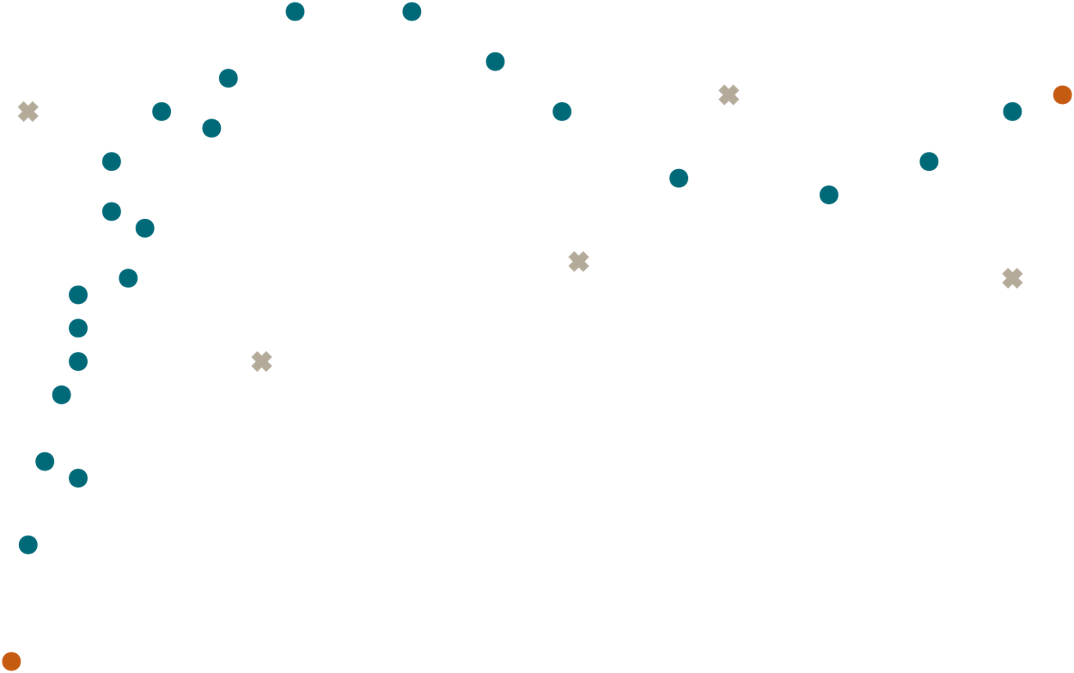
\includegraphics[width=0.8\linewidth]{intuition/state_0}};
		}
		\onslide<2>{
			\node (pointcloud)
			{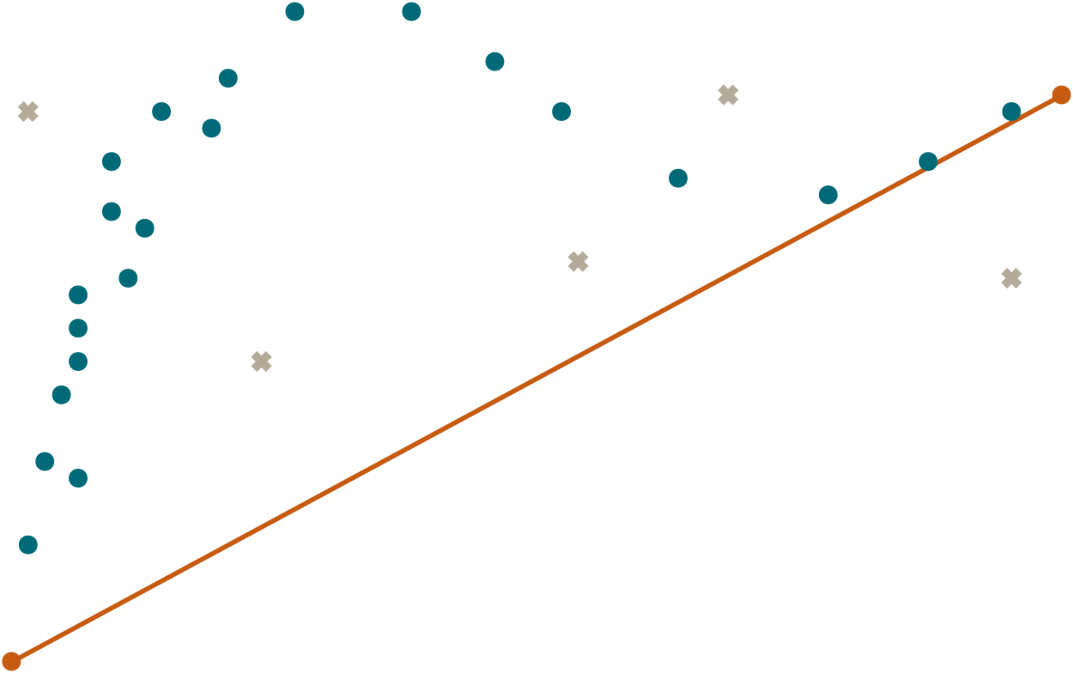
\includegraphics[width=0.8\linewidth]{intuition/state_1}};
		}
		\onslide<3>{
			\node (pointcloud)
			{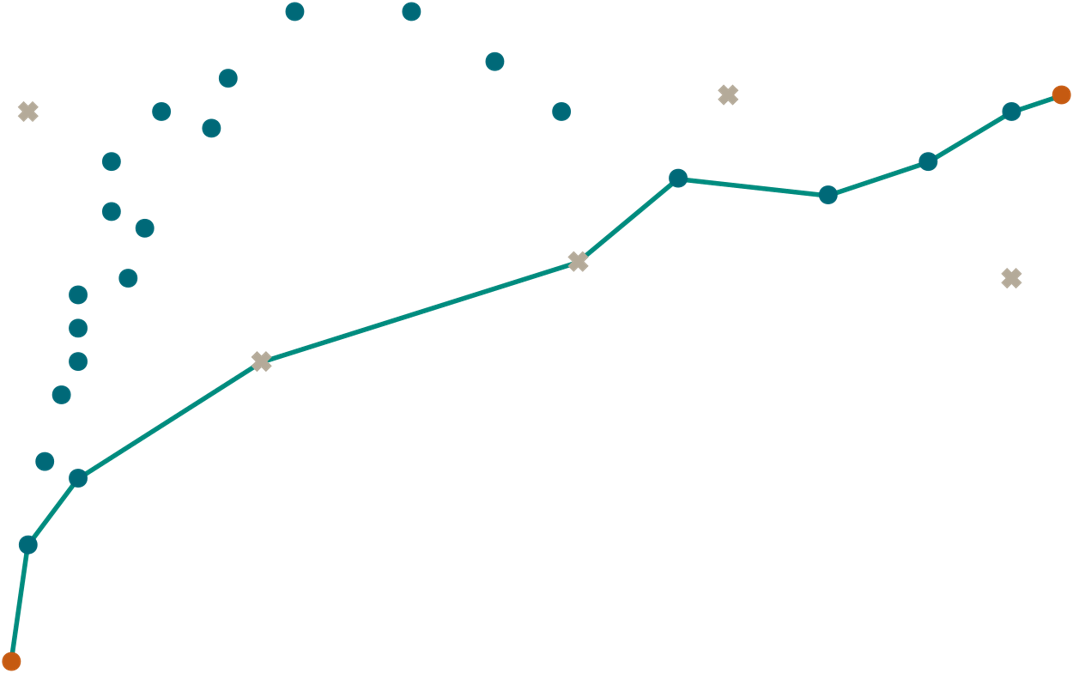
\includegraphics[width=0.8\linewidth]{intuition/state_2}};
		}
		\onslide<4>{
			\node (pointcloud)
			{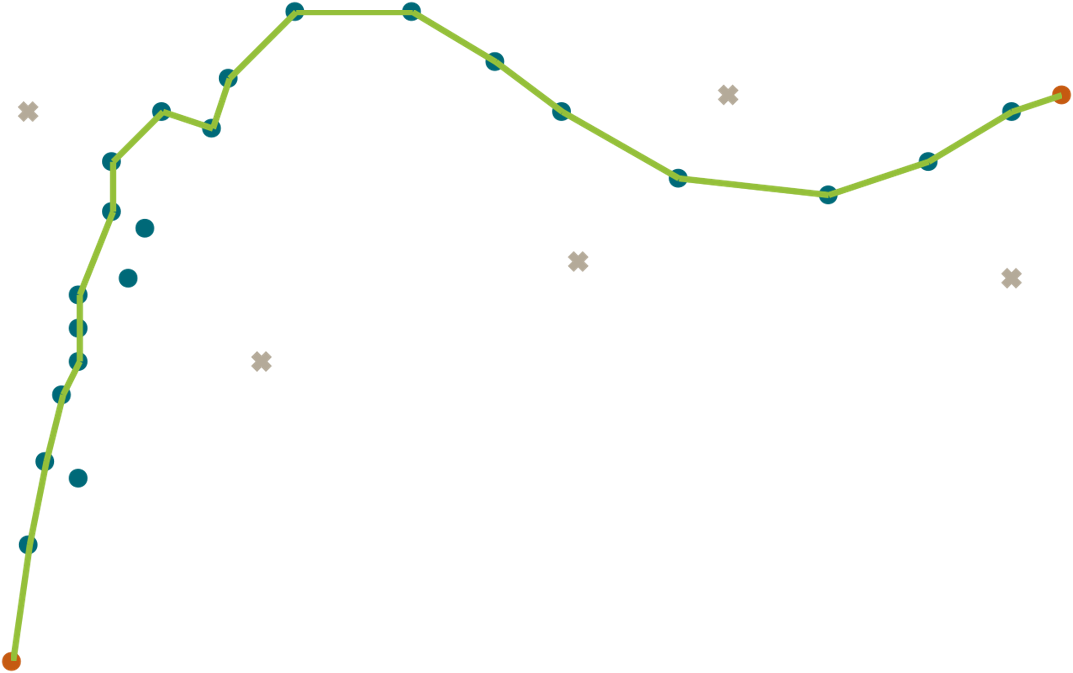
\includegraphics[width=0.8\linewidth]{intuition/state_3}};
		}
		\node[legend, anchor=south east] at (pointcloud.south east){
			\fontsize{\legendsize}{9pt}\selectfont
			\begin{itemize}[itemsep=0pt,partopsep=0pt,topsep=0pt]
				\item[{
\includegraphics[width=\legendsize]{intuition/inlier}}] Inlier
				\item[{
\includegraphics[width=\legendsize]{intuition/endpoint}}] Endpoint
				\item[{
\includegraphics[width=\legendsize]{intuition/outlier}}] Outlier
			\end{itemize}
		};
	\end{tikzpicture}
	
	\vspace*{0.5cm}
	
	\begin{tabular}{ccc}
		\visible<2->{\small\color{pathorange}
		$\min_P \sum_{e \in P} \length(e)^{~}$	
		} & 
		\visible<3->{\small\color{pathblue}
		$\min_P \sum_{e \in P} \length(e)^2$} &
		\visible<4->{\small\color{pathgreen}
		$\min_P \sum_{e \in P} \length(e)^p$
		}
	\end{tabular}
\end{frame}

% Lexicographic order
\begin{frame}[c]{Limit behaviour when $p \rightarrow \infty$}
	Total order on edges based on their length: $e_1 > e_2 > \dots > e_n$
	\pause
	
	There is a $p$ large enough such that, for all $i=1,\dots,n$:
	\[
		\length(e_i)^p > \sum_{j > i} \length(e_j)^p
	\]
	
	\pause
	$\mathcal{P}_1 = \{ e_1, e_2, \cdots, e_m \}$ with $e_1 > e_2 > \cdots > e_m$.
	$\mathcal{P}_2 = \{ e'_1, e'_2, \cdots, e'_p \}$ with $e'_1 > e'_2 > \cdots > e'_p$.
\end{frame}

% Crash course
%\begin{frame}[c]{Simplicial homology}
%	\begin{tabular}{cc}
%		Simplices & \raisebox{-.5\height}{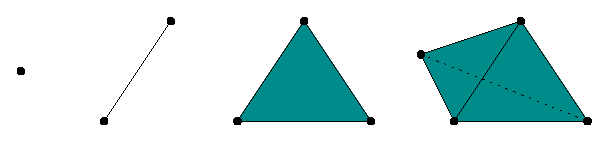
\includegraphics[width=0.5\textwidth]{course/simplices}} \\
%		Simplicial complex & \raisebox{-.5\height}{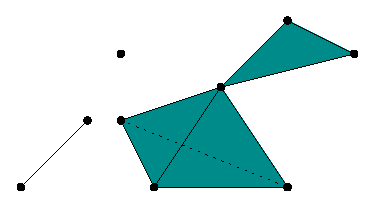
\includegraphics[width=0.4\textwidth]{course/complex}}
%	\end{tabular}
%		
%	\vspace{1cm}
%	
%	A \textbf{\textit{k}-chain} $A$ with coefficients in $\F$ is a formal sum of $k$-simplices:
%	\begin{equation*}
%		A = \sum_{i} x_i \sigma_i, \text{ with } x_i \in \F \; \text{and} \;\sigma_i \in K^{(k)}
%	\end{equation*}
%\end{frame}

%\begin{frame}{Boundary operator}
%	The \textbf{boundary operator} $\partial_k : \Cchains_{k}(K) \to \Cchains_{k-1}(K)$ is the linear map defined for any $k$-simplex $\sigma = [a_0, \dots, a_k]$ as:
%	\[
%	\partial_k \sigma  \defunder{=}\sum_{i=0}^{k} (-1)^{i} [a_0,\dots, \widehat{a_i},\dots, a_k]
%	\]
%	
%	\begin{center}
%		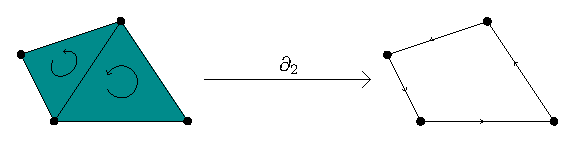
\includegraphics[width=0.8\textwidth]{course/boundary}
%	\end{center}
%\end{frame}
%
%\begin{frame}{Cycles \& Boundaries}
%	The kernels and images of the boundary operator form respectively the vector space of \textbf{cycles} and \textbf{boundaries}:
%	\begin{align*}
%		\Zchains_{k}(K) &\defunder{=} \Ker \partial_k = \Big\{ \Gamma \in \Cchains_{k}(K), \partial_k \Gamma = 0 \Big\} \\
%		\Bchains_k(K) &\defunder{=} \Ima \partial_{k+1} = \Big\{ \Gamma \in \Cchains_{k}(K), \exists A \in \Cchains_{k+1}(K) \mid \Gamma = \partial_{k+1} A \Big\}
%	\end{align*}
%
%	\[
%		\partial_{k} \partial_{k+1} = 0 \iff \Bchains_k(K) \subset \Zchains_k(K)
%	\]
%	
%	\begin{center}
%		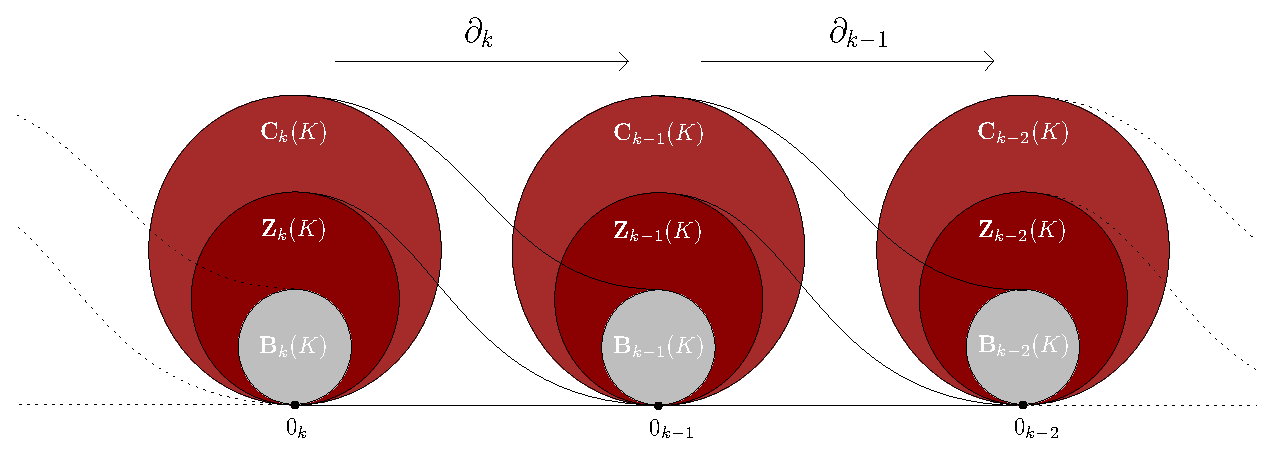
\includegraphics[width=0.7\linewidth]{course/sequence}
%	\end{center}
%\end{frame}

%
%\begin{frame}{Fundamental property}
%	\begin{tabular}{lcl}
%	$\partial_{k} \partial_{k+1} = 0$ && ``Boundaries have no boundaries'' \\
%	\pause
%	& $\iff$ & \\
%	$\Bchains_k(K) \subset \Zchains_k(K)$ && ``All boundaries are cycles''
%	\end{tabular}
%
%	\pause
%	\begin{center}
%		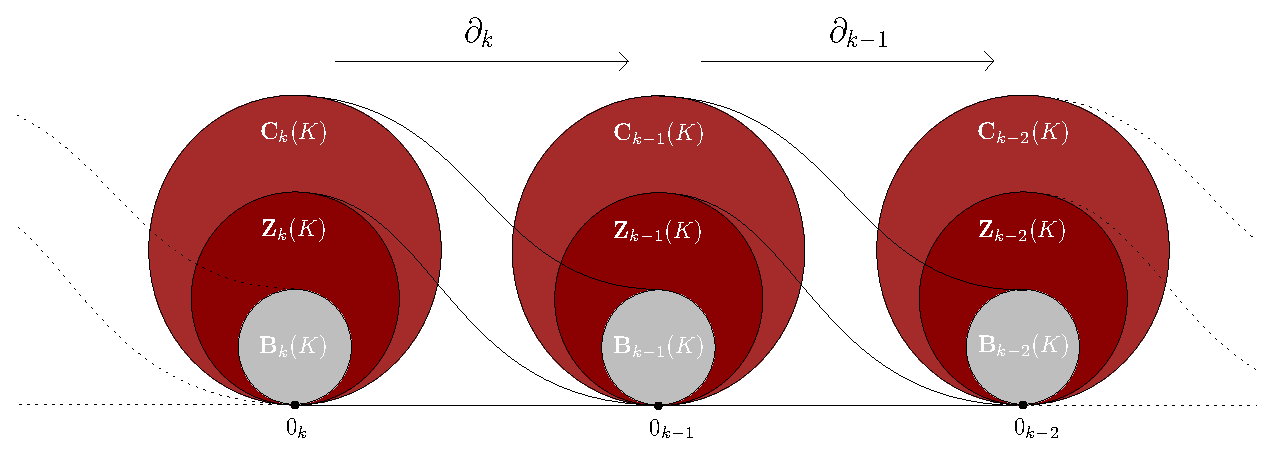
\includegraphics[width=0.9\textwidth]{course/sequence}
%	\end{center}
%\end{frame}

%\begin{frame}{Simplicial homology}
%	\textbf{Homology groups} are defined as quotient spaces of cycles over boundaries:
%	\[
%	\Homol_k(K) \defunder{=} \frac{\Zchains_k(K)}{\Bchains_k(K)}
%	\]
%	
%	$A, A' \in \Zchains_k(K)$ are \textbf{homologous cycles}
%	
%	\pause
%	\vspace*{5pt}
%	
%	\hspace*{5pt} $\defunder{\iff}$ they belong to the same homology class in $\Homol_k(K)$ \\
%	
%	\pause
%	\vspace*{5pt}
%	
%	\hspace*{5pt} $\iff A -  A' = \partial_{k+1}B$ for some ($k+1$)-chain $B$.
%	
%	\begin{center}
%		\begin{tikzpicture}
%			\node[help lines](torus) {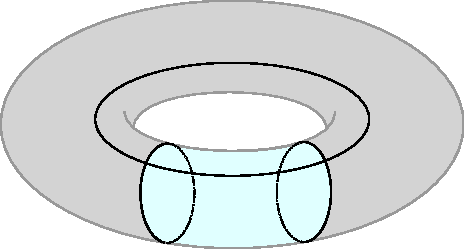
\includegraphics[width=0.5\linewidth]{course/homologous}};
%			\node[below left=-1cm and -1.75cm of torus]{$A$};
%			\node[below right=-1cm and -1.75cm of torus]{$A'$};
%			\node[below=-0.8cm of torus]{$B$};
%			\node[above=-0.8cm of torus]{$C$};
%		\end{tikzpicture}
%	\end{center}
%\end{frame}

% Lexicographic order
\begin{frame}{Lexicographic preorder on chains}
	$K$: simplicial complex.\\
	$\F$: field ($\Z_2$ or $\Q$)\\
	$\Cchains_k(K; \F)$: Vector space of $k$-chains.
	
	\textbf{Total order} on $k$-simplices, denoted $<$.
	
	\textbf{Lexicographic preorder} Given $\Gamma_1, \Gamma_2 \in \Cchains_k(K; \F)$,
	\[
	\Gamma_1 \LexicographicOrderChain \Gamma_2 \defunder{\iff}
	\begin{cases} 
		|\Gamma_1| = |\Gamma_2| \\
		\operatorname{or} \\
		\max \big\{ \sigma \in |\Gamma_1| \triangle |\Gamma_2|  \big\}  \in |\Gamma_2|
	\end{cases}
	\]
	where $\triangle$ denotes the set symmetric difference.
	
	%	\[
	%		\big( \Gamma_1 \LexicographicOrderChain \Gamma_2 \quad \textrm{and} \quad  	\Gamma_2 
	%		\LexicographicOrderChain  \Gamma_1 \big) \iff |\Gamma_1| = |\Gamma_2| 
	%	\]
	%	
	%	\begin{alertblock}{$\F = \Z_2$}
	%		$\LexicographicOrderChain$ is a total order.
	%	\end{alertblock}
\end{frame}

% Total order on k-simplices
\begin{frame}[c]{A total order based on the Delaunay triangulation (I)}
	\scriptsize
	\begin{block}{\scriptsize Total order on 2-simplices}
		For $\sigma_1, \sigma_2 \in K^{(2)}$,
		\[
		\sigma_1 \leq \sigma_2 \defunder{\iff}
		\begin{cases}
			\rseb(\sigma_1) < \rseb(\sigma_2) &\\
			\:  \operatorname{or} &\\
			\rseb(\sigma_1) = \rseb(\sigma_2) & \operatorname{and} \circrad(\sigma_1) \geq \circrad(\sigma_2)
		\end{cases}
		\]
	\end{block}
	
	\begin{center}
		\begin{minipage}{0.5\linewidth}
			\centering
			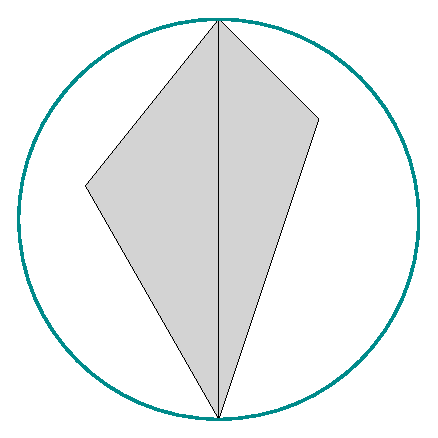
\includegraphics[height=0.3\textheight]{order_rseb}\\
			\color{pathblue}$\rseb(\sigma_1) = \rseb(\sigma_2)$	
		\end{minipage}%
		\begin{minipage}{0.5\linewidth}
			\centering
			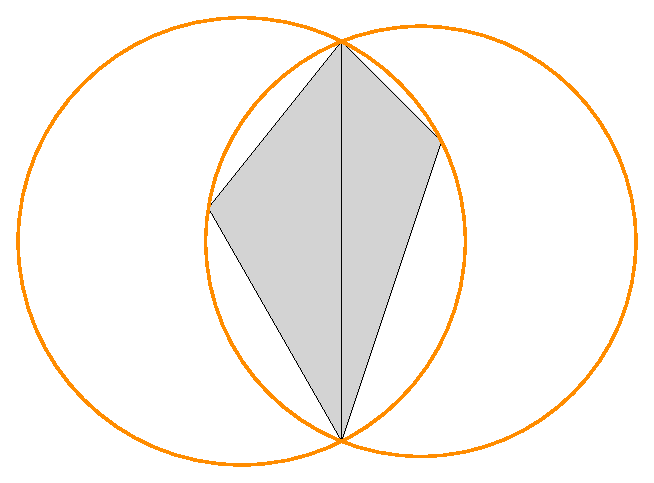
\includegraphics[height=0.3\textheight]{order_rcirc}\\
			\color{pathorange} $\circrad(\sigma_1) \neq \circrad(\sigma_2)$
		\end{minipage}%
	\end{center}
\end{frame}

\begin{frame}{A total order based on the Delaunay triangulation (II)}
	\small
	\begin{minipage}{0.6\linewidth}
		\begin{block}{\small Proposition}
			The support of
			\[
			\min_{\LexicographicOrderChain} \{ \Gamma \in \Cchains_2(K), \partial \Gamma = \beta_{\mathbf{P}} \}
			\]
			corresponds to the $2$-simplices of the Delaunay triangulation of $P$.
		\end{block}
	\end{minipage}%
	\begin{minipage}{0.4\linewidth}
		\begin{tikzpicture}
			\node (delaunay) { 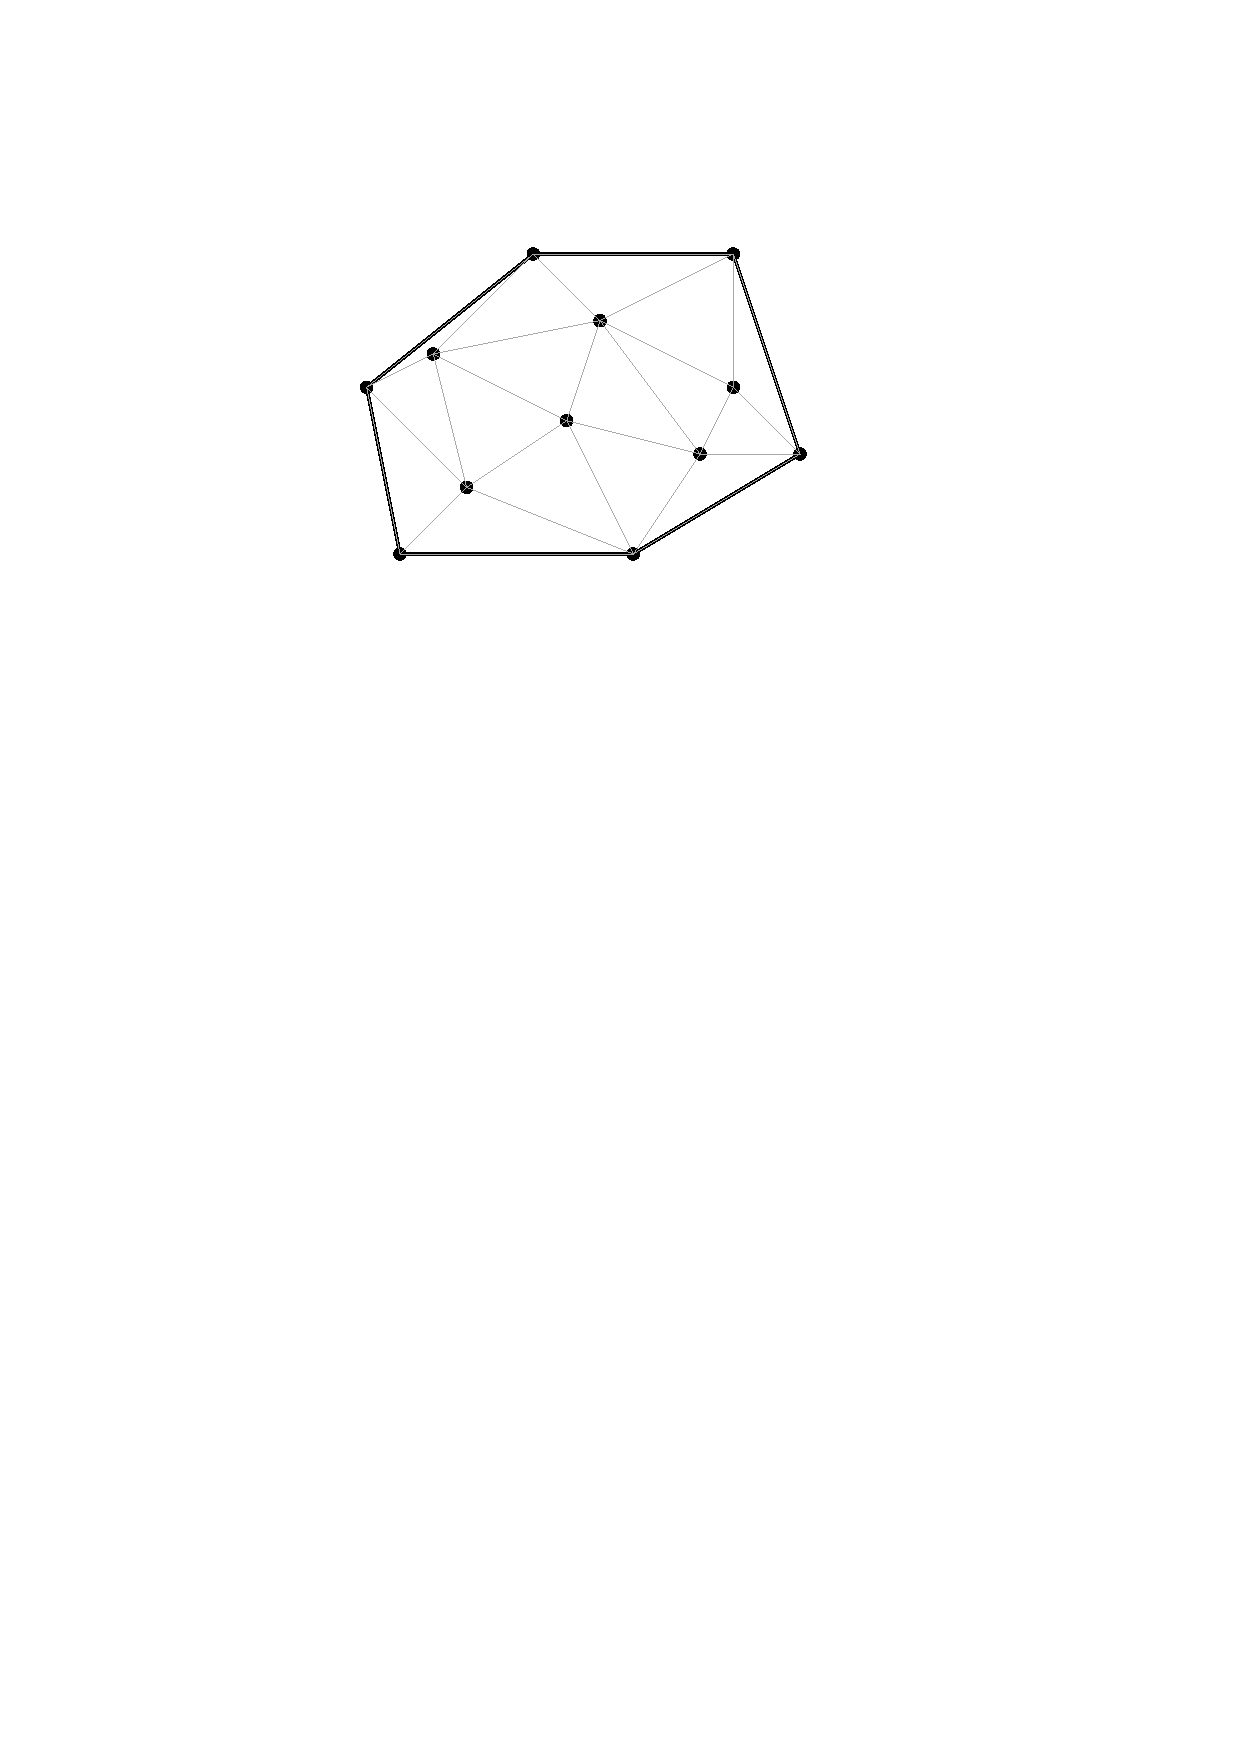
\includegraphics[width=0.9\linewidth]{delaunay_bp} };
			\node[above right=-0.5cm and -0.5cm of delaunay]{$\beta_{\mathbf{P}}$};
			\node at (0.2cm, 0) {$\mathbf{P}$};
		\end{tikzpicture}
	\end{minipage}
	
	\vspace{0.5cm}
	
	\textbf{Generalization} of a total order for simplices in any dimension.
	
	\textbf{Characterization of regular triangulations} as lexicographic optimal chains.
\end{frame}

% Formulation
\begin{frame}{Homological formulation}
\scriptsize

\begin{minipage}[c]{0.55\linewidth}
\textbf{Optimal homologous chain} to a given chain $\alpha$
\begin{equation*}
	\alpha_{\min} = \min \Big\{ \alpha + \partial_{k+1} B, \: A \in \Cchains_{k+1}(K) \Big\}
\end{equation*}

\textbf{Optimal chain under imposed boundary} $\beta$
\begin{equation*}
	\Gamma_{\min} = \min \Big\{ \Gamma \in \Cchains_k(K) \mid \partial_k \Gamma = \beta \Big\}
\end{equation*}
\end{minipage}%
\hfill%
\begin{minipage}[c]{0.40\linewidth}
	\begin{tikzpicture}
		\node(image){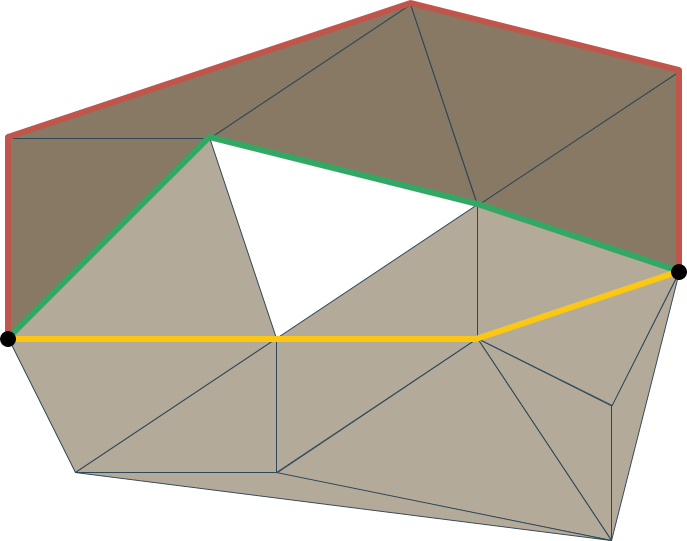
\includegraphics[width=\linewidth]{problems}};
		\node[homred, above=-0.2cm of image]{$\alpha$};
		\node[homgreen, above left=-1.7cm and -2.5cm of image]{$\alpha_{\min}$};
		\node[above left=-2.5cm and 0cm of image]{$\beta$};
		\node[homyellow, below left=-1.2cm and -1.5cm of image]{$\Gamma_{\min}$};
	\end{tikzpicture}
\end{minipage}

\pause
\vspace{1cm}
\textbf{NP-hard} for L1 minimization \cite{chen_HardnessResultsHomology_2011} \\
\pause
\textbf{Polynomial algorithms} for lexicographic optimality.
\end{frame}

% Formulation: Imposed boundary
\begin{frame}{Polynomial algorithms}
	\small
	
	\textbf{Boundary matrix}
	\[
		\partial_{k+1} = \arrowbounded{\begin{pmatrix}
				0 & 1 & 1 \\
				1 & 0 & 1 \\
				1 & 1 & 1 \\
				1 & 1 & 0 \\
		\end{pmatrix}
		}{Arbitrary order on (k+1)-simplices} \text{\tiny Total order on k-simplices}
	\]
	
	\vspace{0.2cm}
	
	\textbf{Matrix reduction algorithm} for persistent homology \cite{edelsbrunner_ComputationalTopologyIntroduction_2010}
	
	\textbf{Time complexity:} $\BigO(n^3)$ 
\end{frame}

%\begin{frame}{Properties after matrix reduction}
%	\small
%	
%	\[
%		\alpha \text{ is reducible by } \beta \defunder{\iff} \begin{cases}
%			\beta \text{ homologous to } \alpha \\
%			\beta \LexicographicStrictOrderChain \alpha
%		\end{cases}
%	\]
%	
%	\begin{block}{\small Property 1}
%		A chain is reducible iff one of its simplices is reducible.
%	\end{block}
%	
%	
%	\begin{block}{\small Property 2}
%		There is a 1-to-1 correspondence between reducible simplices and non-zero columns of the reduced matrix.
%	\end{block}
%	
%	\begin{center}
%	$R = $\begin{tikzpicture}[baseline=-0.5ex]
%		\matrix (boundary)[matrix of math nodes, ampersand replacement=\&, left delimiter={(},right delimiter={)}]{
%			0 \& 1 \& 1 \\
%			1 \& 1 \& 1 \\
%			1 \& 0 \& 1 \\
%			1 \& 0 \& 0 \\
%		};
%		\draw[thick,pathorange]($(boundary-4-1.south west)+(0.05, 0.05)$) rectangle ($(boundary-4-1.north east)-(0.05, 0.05)$);
%		\draw[thick,pathblue]($(boundary-3-1.south west)+(0.05, 0.05)$) rectangle ($(boundary-1-1.north east)-(0.05, 0.05)$);
%		
%		\draw[thick,pathorange]($(boundary-2-2.south west)+(0.05, 0.05)$) rectangle ($(boundary-2-2.north east)-(0.05, 0.05)$);
%		\draw[thick,pathblue]($(boundary-1-2.south west)+(0.05, 0.05)$) rectangle ($(boundary-1-2.north east)-(0.05, 0.05)$);
%
%		\draw[thick,pathorange]($(boundary-3-3.south west)+(0.05, 0.05)$) rectangle ($(boundary-3-3.north east)-(0.05, 0.05)$);
%		\draw[thick,pathblue]($(boundary-2-3.south west)+(0.05, 0.05)$) rectangle ($(boundary-1-3.north east)-(0.05, 0.05)$);
%		
%		\node[below right=-0.8cm and 0.5cm of boundary]{\color{pathorange}Reducible simplex};
%		\node[above right=-0.8cm and 0.5cm of boundary]{\color{pathblue} Reductions};	
%	\end{tikzpicture}
%	\end{center}
%
%\end{frame}

% Efficient version
\begin{frame}{Efficient versions in codimension 1}
\scriptsize

\textbf{Simplicial complex}: $d$-pseudomanifold $\M$.\\
\textbf{Codimension 1}: Looking for $(d-1)$-chains.
\vspace{0.2cm}

\pause

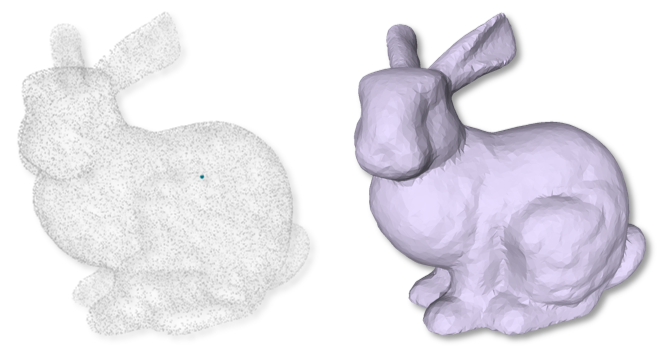
\includegraphics[width=0.47\linewidth]{applications/bunny}%
\hfill
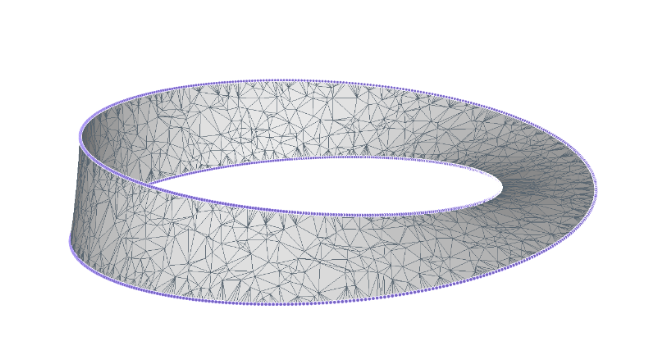
\includegraphics[width=0.47\linewidth]{applications/mobius}
\vspace{0.2cm}

\begin{minipage}{0.47\linewidth}
\textbf{Closed surface reconstruction}\\
Given two distinct $d$-simplices ($\tau_1, \tau_2)$ of $\M$, find the lexicographic optimal $(d-1)$-chain homologous to $\partial\tau_1$ in $\M \setminus \{ \tau_1, \tau_2 \}$.
\end{minipage}%
\hfill
\begin{minipage}{0.47\linewidth}
\textbf{Open surface reconstruction}\\
Given a $(d-2)$-boundary $A$ in $\M$, find the lexicographic optimal $(d-1)$-chain bounded by $A$ in $\M$.
\end{minipage}
\end{frame}


\begin{frame}{Closed surface: dual formulation}
\small
\begin{center}
\begin{tabularx}{\linewidth}{@{}YYY@{}}
\visible<1->{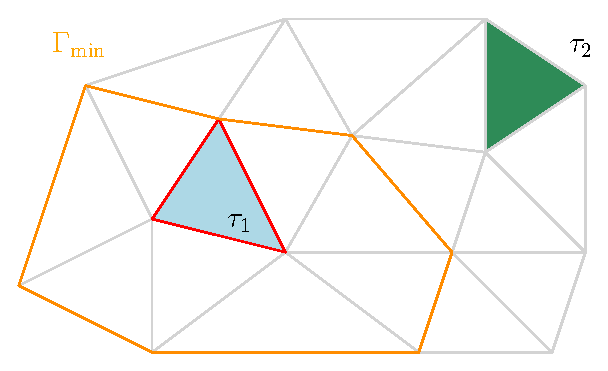
\includegraphics[width=\linewidth]{dual/primal_problem}}
& \visible<2->{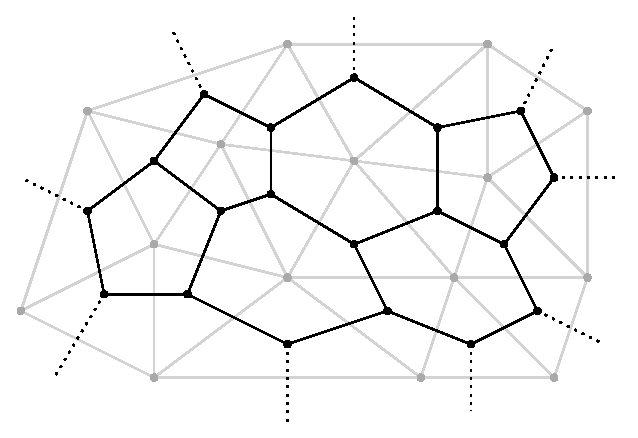
\includegraphics[width=\linewidth]{dual/dual_graph}}
& \visible<3->{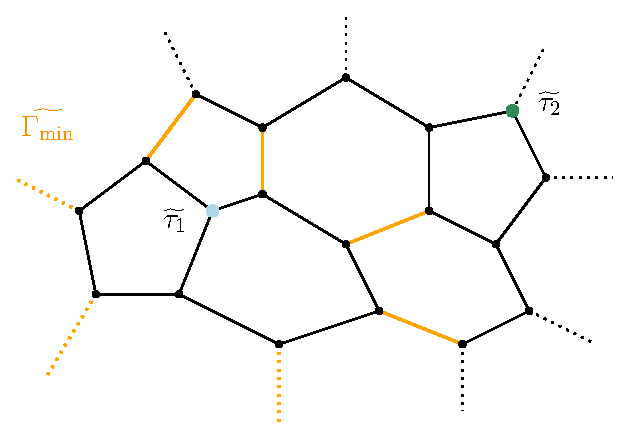
\includegraphics[width=\linewidth]{dual/dual_problem}} \\
\visible<1->{Primal problem} & \visible<2->{Duality} & \visible<3->{Dual problem}
\end{tabularx}
\end{center}

\visible<3->{
	\textbf{Lexicographic mincut}\\
	Given a dual graph $G=(\GraphV, \GraphE)$, two vertices $\widetilde{\tau}_1,\widetilde{\tau}_2 \in \GraphV$, find the set $\widetilde{\Gamma}_{\operatorname{LMC}} \subset \GraphE$ minimal for the lexicographic order $\LexicographicOrderChain$, that  disconnects $\widetilde{\tau}_1$ and $\widetilde{\tau}_2$ in $G$.
}
\end{frame}

\begin{frame}{Disjoint-sets structure}
	Parent-tree representation for sets.
	\begin{figure}
		\centering%
		\begin{subfigure}{0.45\textwidth}
			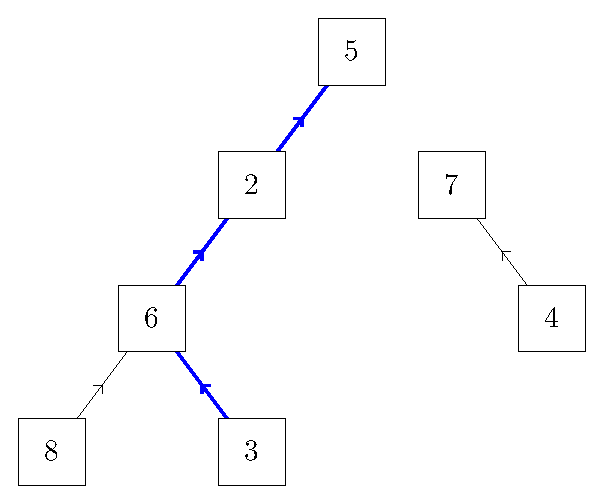
\includegraphics[width=\linewidth]{ds/disjoint_find}
			\subcaption*{\FindSet{$3$} $\rightarrow 5$}
		\end{subfigure}%
		\hspace{0.045\textwidth}%
		\vline%
		\hspace{0.045\textwidth}%
		\begin{subfigure}{0.45\textwidth}
			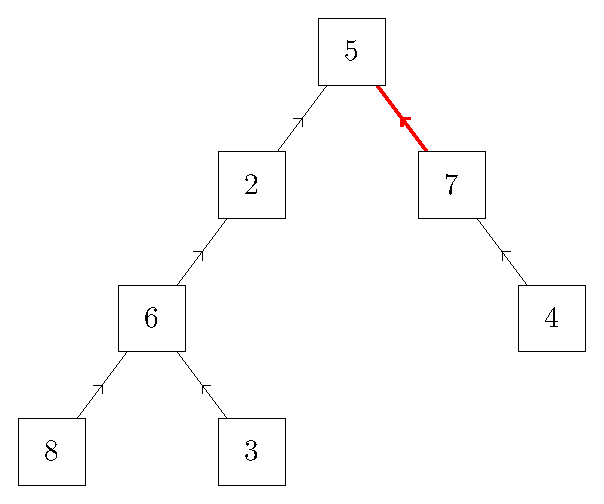
\includegraphics[width=\linewidth]{ds/disjoint_link}
			\subcaption*{\LinkSet{$7$, $5$}}
		\end{subfigure}%
	\end{figure}
	\pause
	\textbf{Complexity: } $\BigO(\alpha(n))$ 
\end{frame}

% Codimension 1: Algorithm
\begin{frame}[c]{Efficient closed surface reconstruction (codimension 1)}
	\scriptsize
	\begin{minipage}[c]{0.5\linewidth}
		\begin{algorithm}[H]
			\SetKwInOut{Input}{Inputs}
			\SetKwInOut{Output}{Output}
			\SetKw{Continue}{continue}
			\SetKw{Or}{or}
			\Input{$\widetilde{\tau_1}, \widetilde{\tau_2} \in \GraphV$}
			
			\alert<0>{$\Gamma_{\operatorname{LMC}} \leftarrow \varnothing$ \\
				\For{$v \in \GraphV$} {
					\MakeSet{$v$}
			}}
			
			\For{$e \in \GraphE$ in decreasing order}{
				$e = (v_1, v_2) \in \GraphV\times \GraphV$ \\
				$r_1 \leftarrow $\FindSet{$v_1$} \\
				$r_2 \leftarrow $\FindSet{$v_2$} \\
				\eIf{$\{ r_1, r_2\} = \{ \widetilde{\tau_1}, \widetilde{\tau_2} \}$}{
					$\Gamma_{\operatorname{LMC}} \leftarrow \Gamma_{\operatorname{LMC}} \cup e$
				}
				{
					\LinkSet{$r_1$, $r_2$}
				}
			}
		\end{algorithm}
	\end{minipage}%
	\begin{minipage}[c]{0.5\linewidth}
		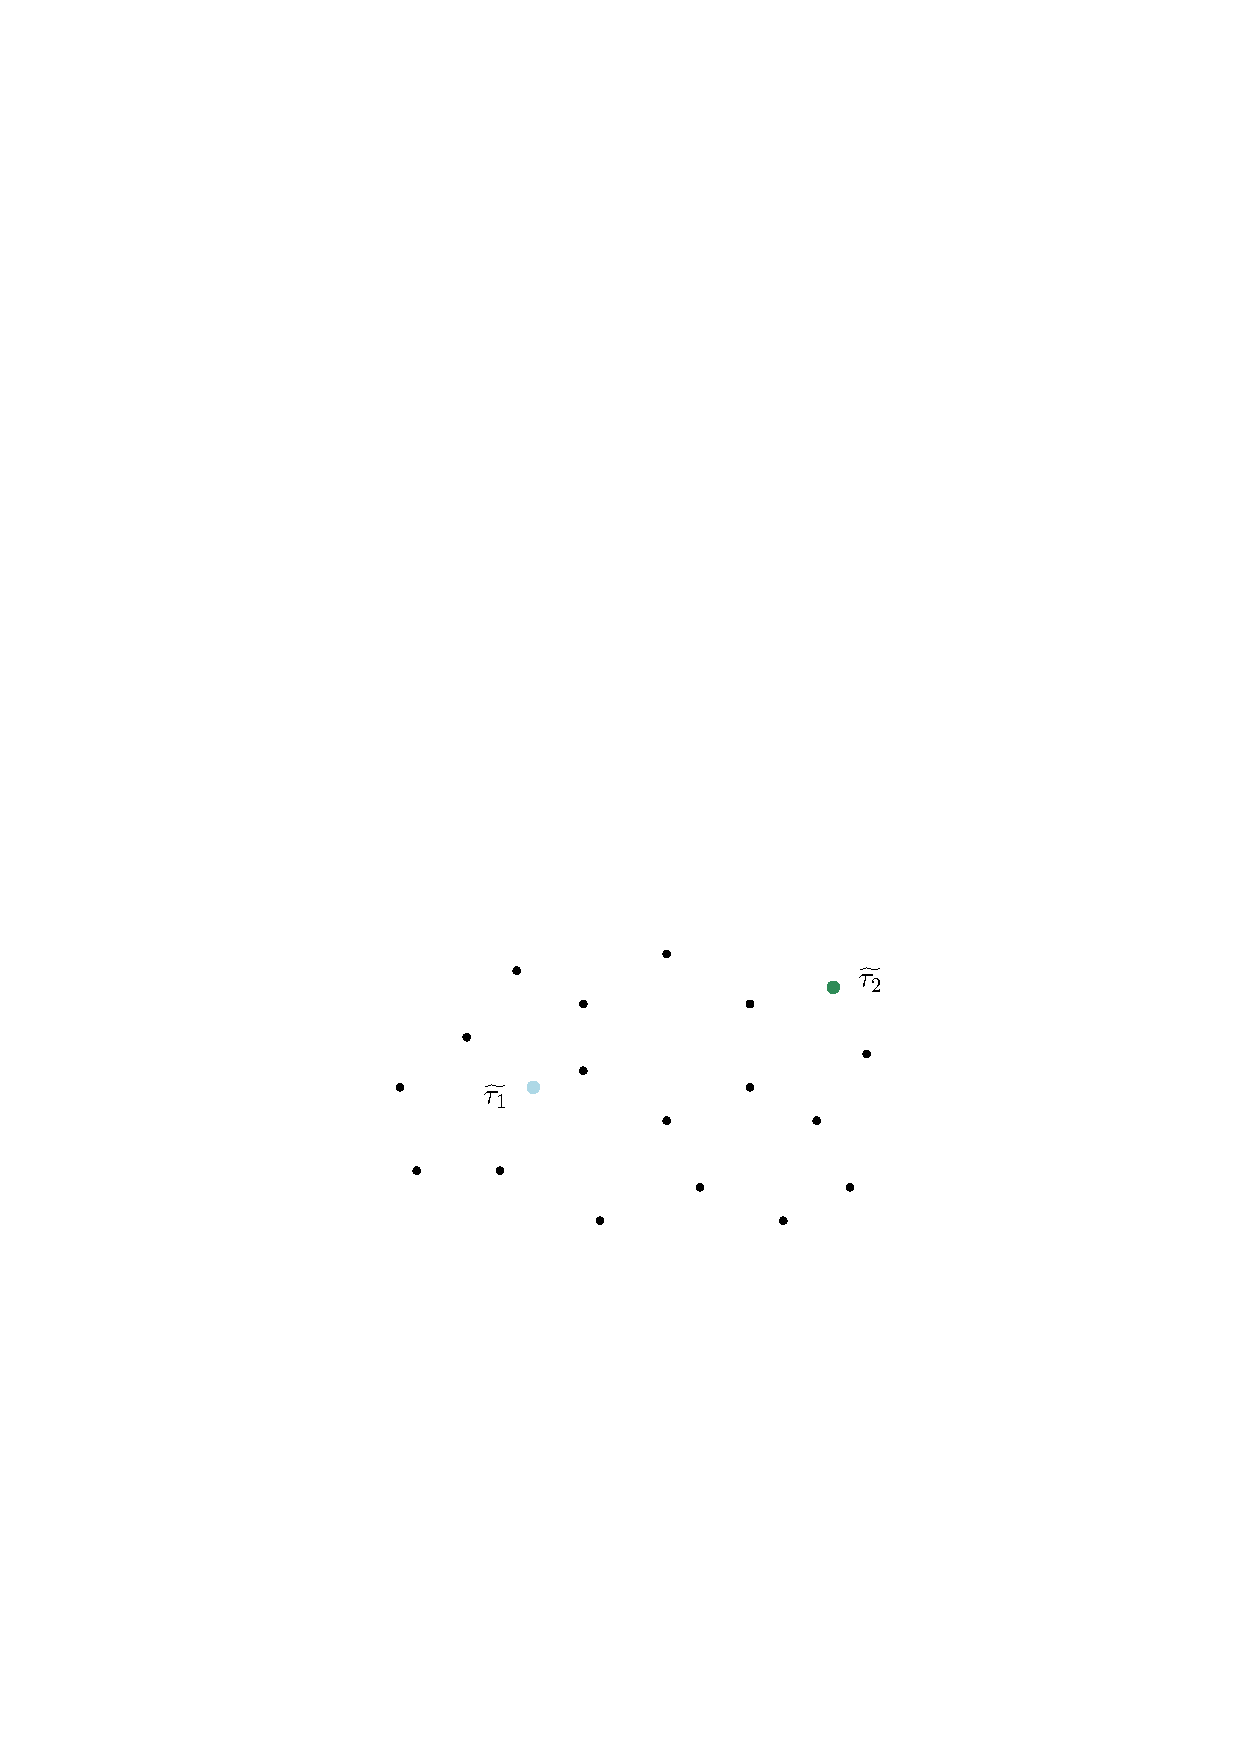
\includegraphics[width=\linewidth]{dual/algo_init}
	\end{minipage}
	
	\textbf{Complexity:} Sorting dual edges ($\BigO(n \log n)$) + Algorithm ($\BigO(n \alpha(n))$).
\end{frame}

\begin{frame}[c]{Efficient closed surface reconstruction (codimension 1)}
	\scriptsize
	\begin{minipage}[c]{0.5\linewidth}
		\begin{algorithm}[H]
			\SetKwInOut{Input}{Inputs}
			\SetKwInOut{Output}{Output}
			\SetKw{Continue}{continue}
			\SetKw{Or}{or}
			\Input{$\widetilde{\tau_1}, \widetilde{\tau_2} \in \GraphV$}

			$\Gamma_{\operatorname{LMC}} \leftarrow \varnothing$ \\
			\For{$v \in \GraphV$} {
					\MakeSet{$v$}
			}
			
			\For{$e \in \GraphE$ in decreasing order}{
				\alert<0|handout:0>{$e = (v_1, v_2) \in \GraphV\times \GraphV$} \\
				\alert<1|handout:0>{$r_1 \leftarrow $\FindSet{$v_1$} \\
									$r_2 \leftarrow $\FindSet{$v_2$} \\
			    }
				\eIf{\alert<2|handout:0>{$\{ r_1, r_2\} = \{ \widetilde{\tau_1}, \widetilde{\tau_2} \}$}}{
					$\Gamma_{\operatorname{LMC}} \leftarrow \Gamma_{\operatorname{LMC}} \cup e$
				}
				{
					\alert<3|handout:0>{\LinkSet{$r_1$, $r_2$}}
				}
			}
		\end{algorithm}
	\end{minipage}%
	\begin{minipage}[c]{0.5\linewidth}
		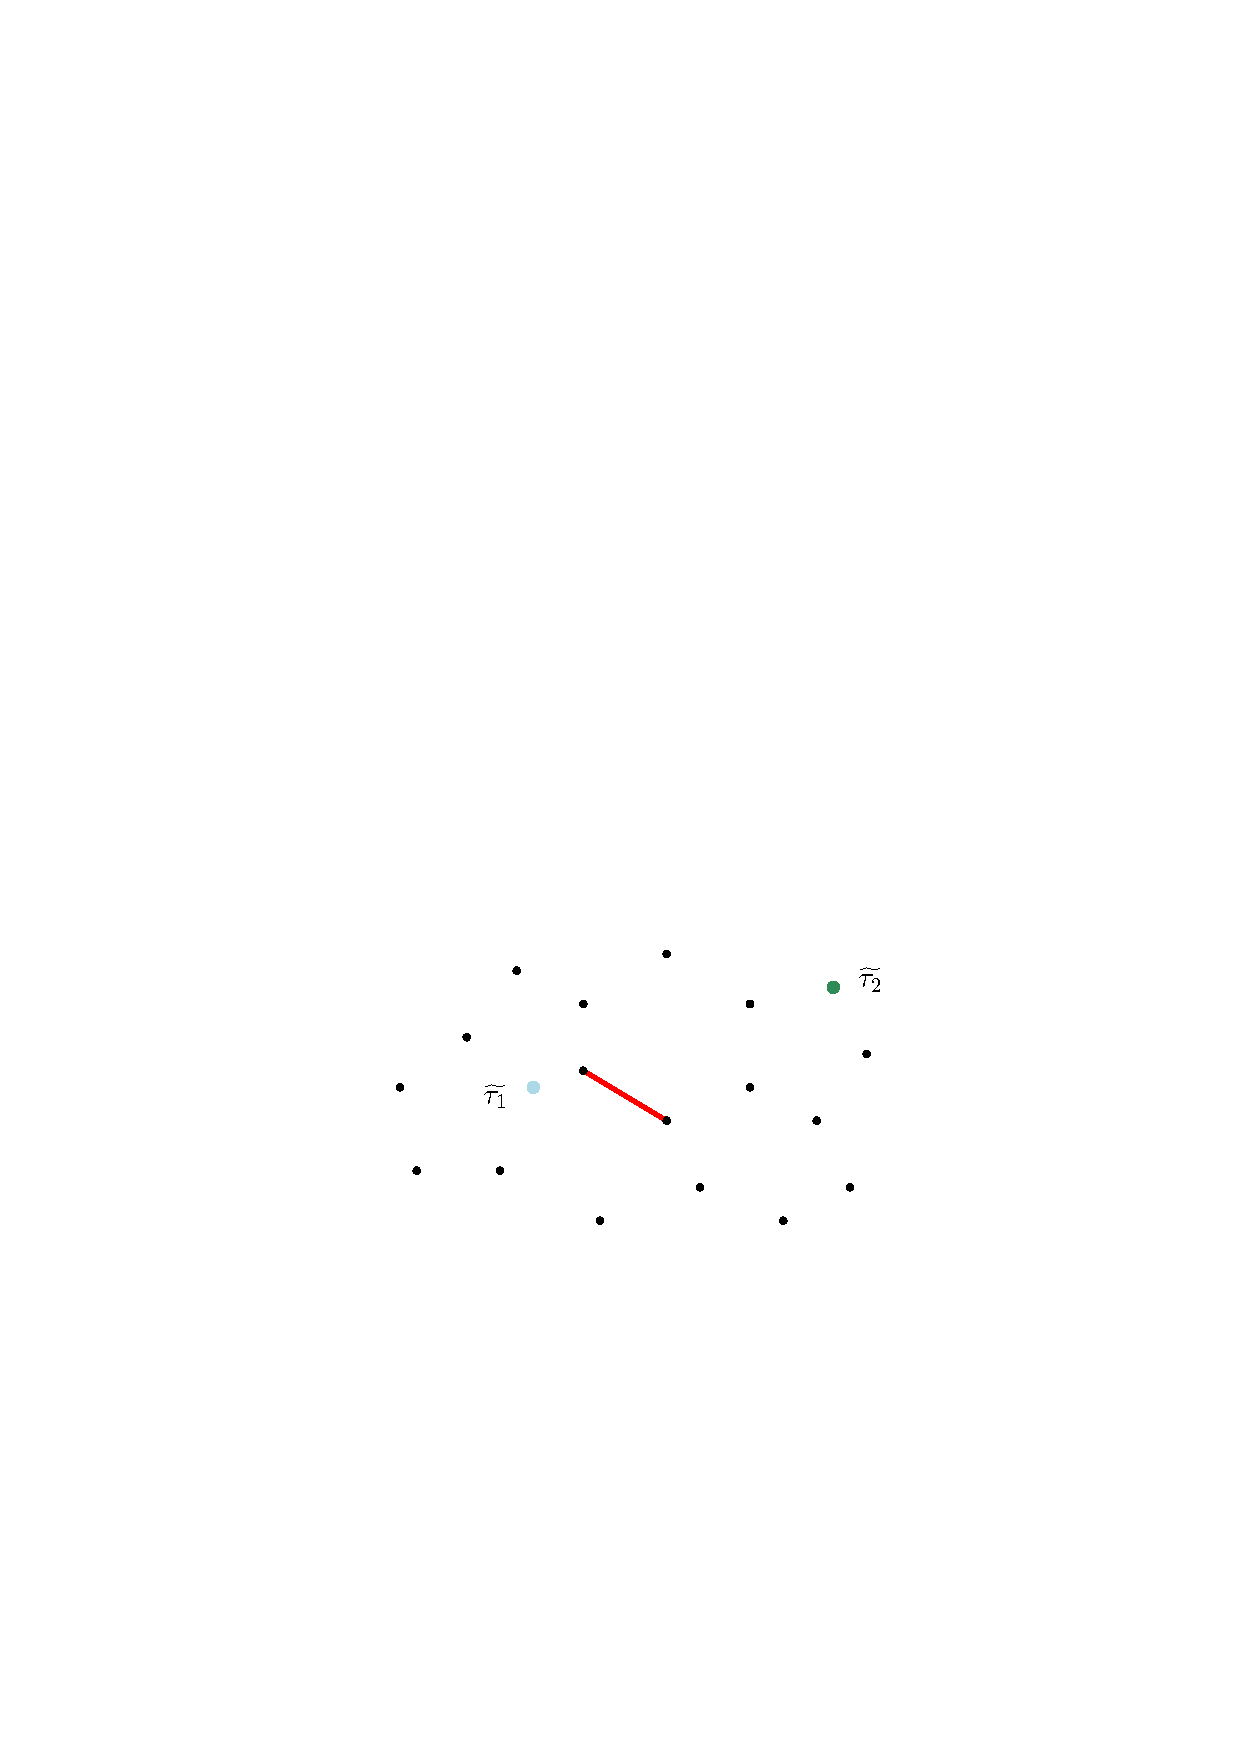
\includegraphics[width=\linewidth]{dual/algo_step1}
	\end{minipage}

	\textbf{Complexity:} Sorting dual edges ($\BigO(n \log n)$) + Algorithm ($\BigO(n \alpha(n))$).
\end{frame}

\begin{frame}[c]{Efficient closed surface reconstruction (codimension 1)}
	\scriptsize
	\begin{minipage}[c]{0.5\linewidth}
		\begin{algorithm}[H]
			\SetKwInOut{Input}{Inputs}
			\SetKwInOut{Output}{Output}
			\SetKw{Continue}{continue}
			\SetKw{Or}{or}
			\Input{$\widetilde{\tau_1}, \widetilde{\tau_2} \in \GraphV$}
			
			$\Gamma_{\operatorname{LMC}} \leftarrow \varnothing$ \\
				\For{$v \in \GraphV$} {
					\MakeSet{$v$}
			}
			
			\For{$e \in \GraphE$ in decreasing order}{
				$e = (v_1, v_2) \in \GraphV\times \GraphV$ \\
				\alert<1|handout:0>{$r_1 \leftarrow $\FindSet{$v_1$} \\
					$r_2 \leftarrow $\FindSet{$v_2$} \\
				}
				\eIf{\alert<2|handout:0>{$\{ r_1, r_2\} = \{ \widetilde{\tau_1}, \widetilde{\tau_2} \}$}}{
					\alert<3|handout:0>{$\Gamma_{\operatorname{LMC}} \leftarrow \Gamma_{\operatorname{LMC}} \cup e$}
				}
				{
					\LinkSet{$r_1$, $r_2$}
				}
			}
		\end{algorithm}
	\end{minipage}%
	\begin{minipage}[c]{0.5\linewidth}
		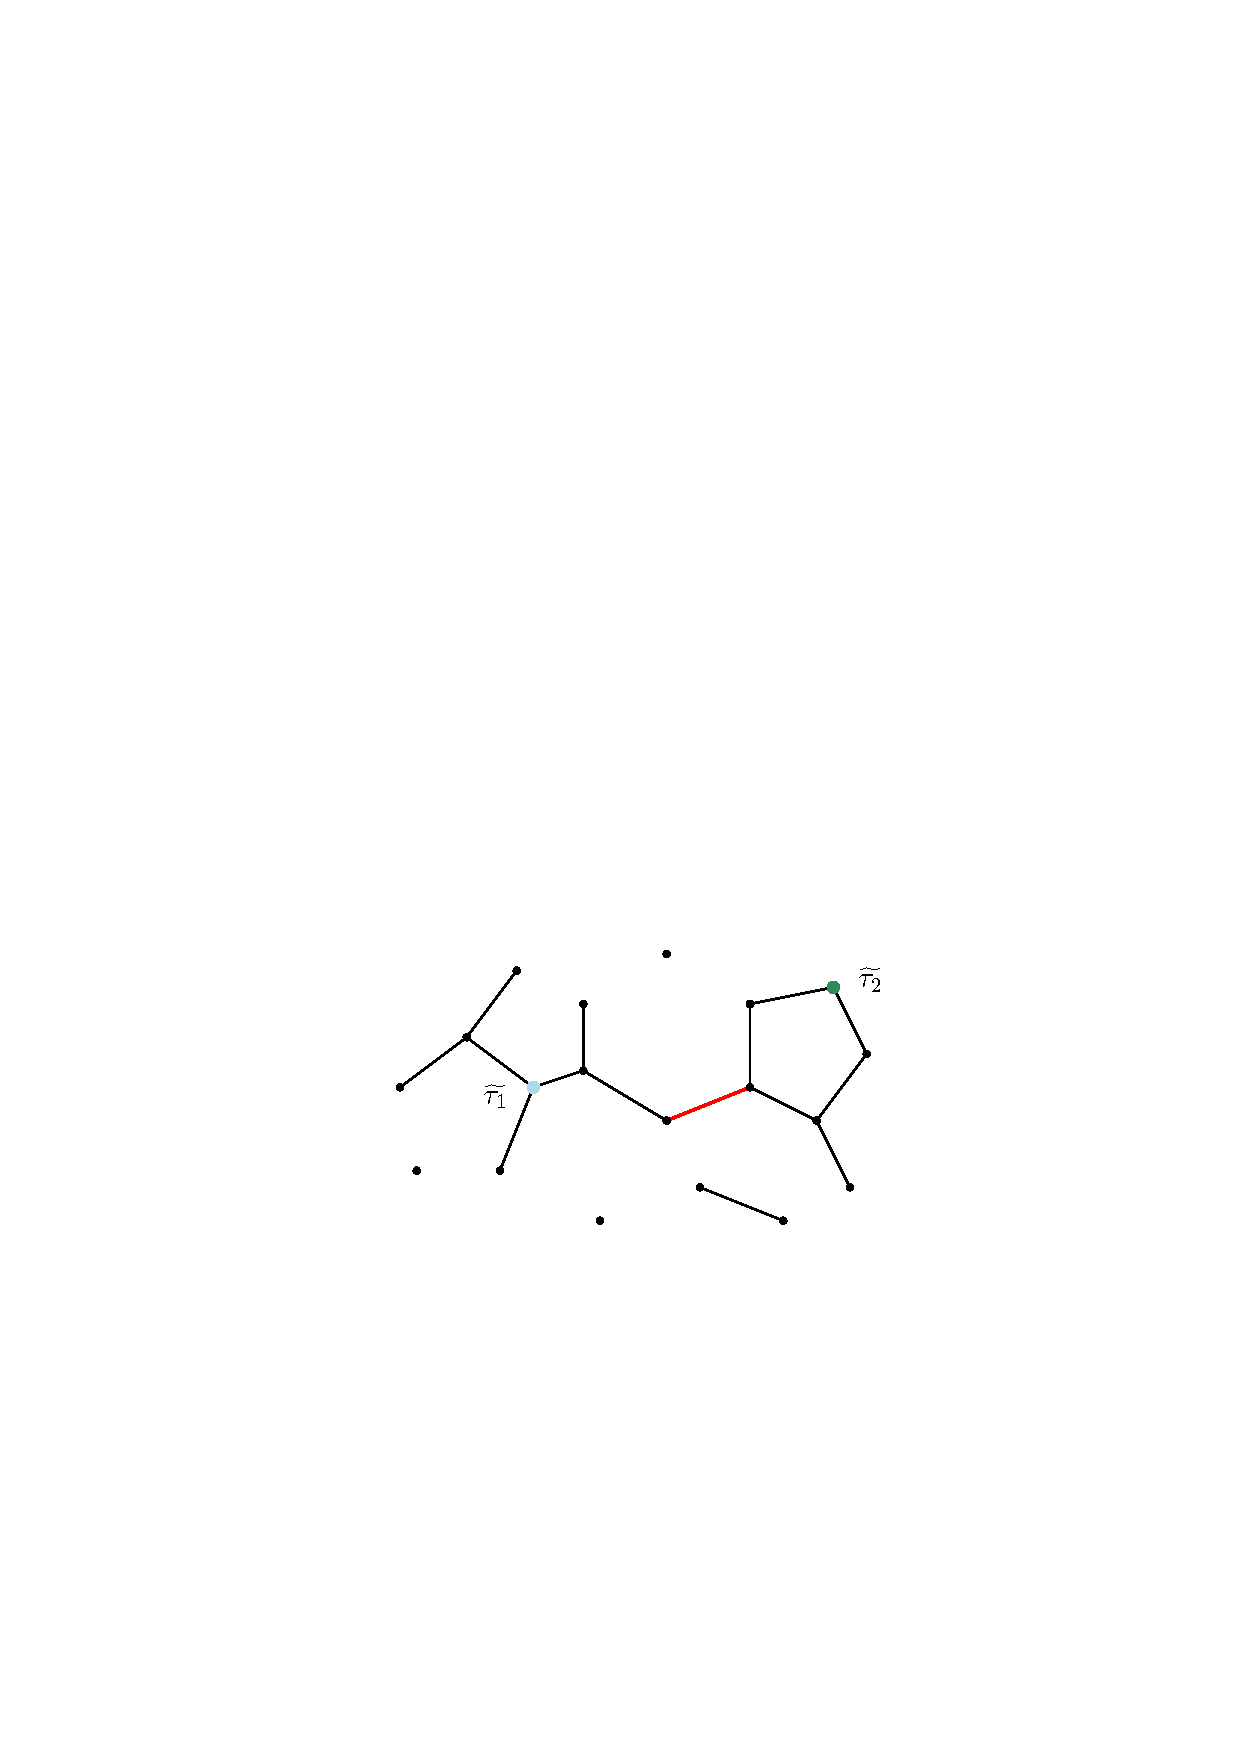
\includegraphics[width=\linewidth]{dual/algo_step2}
	\end{minipage}
	
	\textbf{Complexity:} Sorting dual edges ($\BigO(n \log n)$) + Algorithm ($\BigO(n \alpha(n))$).
\end{frame}

\begin{frame}{Results}
		\begin{center}
			\animategraphics[loop,width=0.49\linewidth]{10}{applications/noisy/}{00001}{00100}%
			\hfill
			\animategraphics[loop,width=0.49\linewidth]{10}{applications/meshed/}{00001}{00100}
		\end{center}
\end{frame}

%\begin{frame}{Relative chains}
%	\textbf{Relative homology} of a simplicial pair $(K, B)$  ``ignores'' all the part of $K$ inside of $B$.
%	\pause
%	\[
%	\Cchains_k(K, B) \defunder{=} \frac{\Cchains_k(K)}{\Cchains_k(B)} 
%	\]
%	\pause
%	%
%	\[
%	\begin{aligned}
%		\Gamma + \Cchains_k(B) \in \Zchains_{k}(K, B) &\iff | \partial_k\Gamma | \subset B\\
%		\Gamma + \Cchains_k(B) \in \Bchains_k(K, B) &\iff  \exists A \in \Cchains_{k+1}(K), |\Gamma - \partial_{k+1} A| \subset B
%	\end{aligned}
%	\]
%	
%	\begin{center}
%		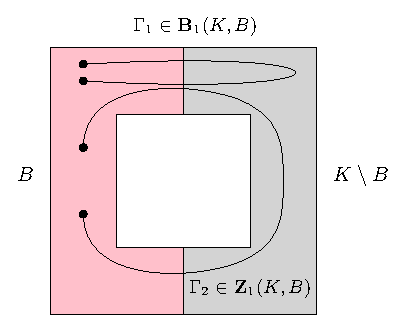
\includegraphics[width=0.4\linewidth]{course/relative_homology}
%	\end{center}
%\end{frame}

\begin{frame}{Efficient open surface reconstruction (codimension 1)}
	\begin{figure}
		\centering
		\small
		\begin{tikzpicture}
			\centering
			\node(inputs){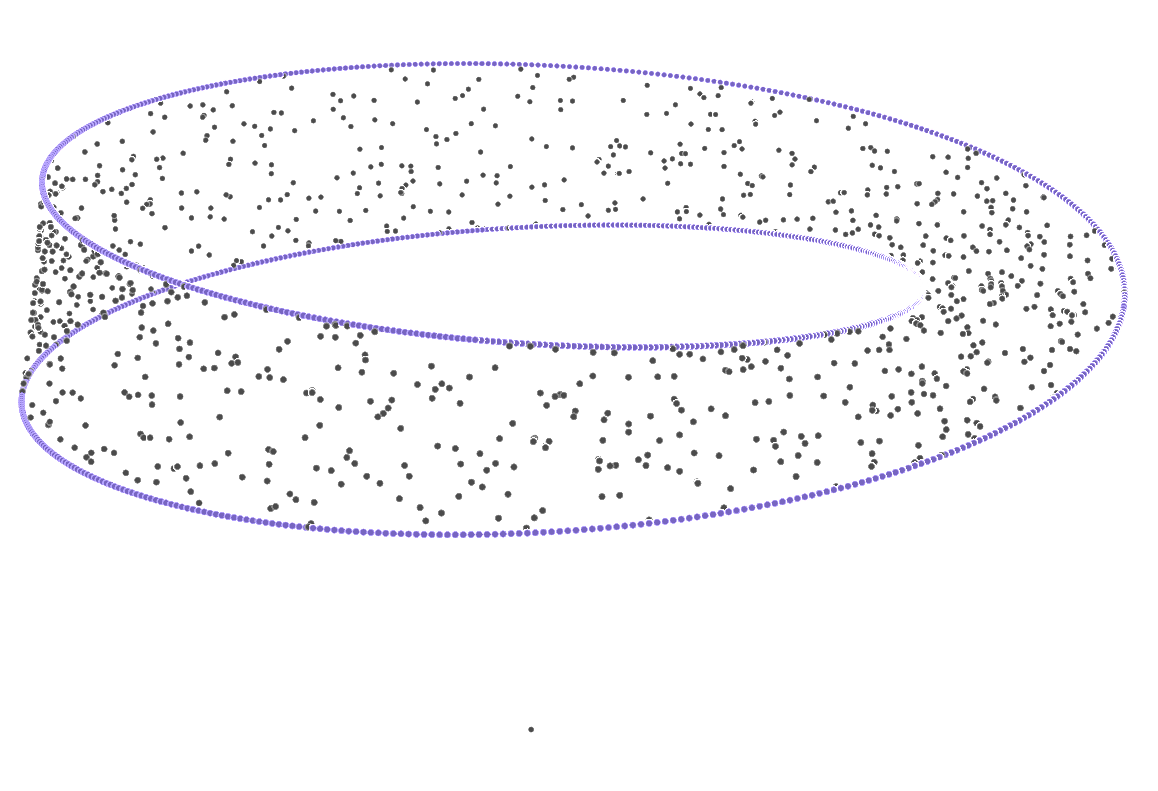
\includegraphics[width=0.32\textwidth]{applications/mobius-points}};
			\node[below=0cm of inputs]{Inputs};
		\end{tikzpicture}%
		\visible<2->{%
		\begin{tikzpicture}
			\centering
			\node(rep){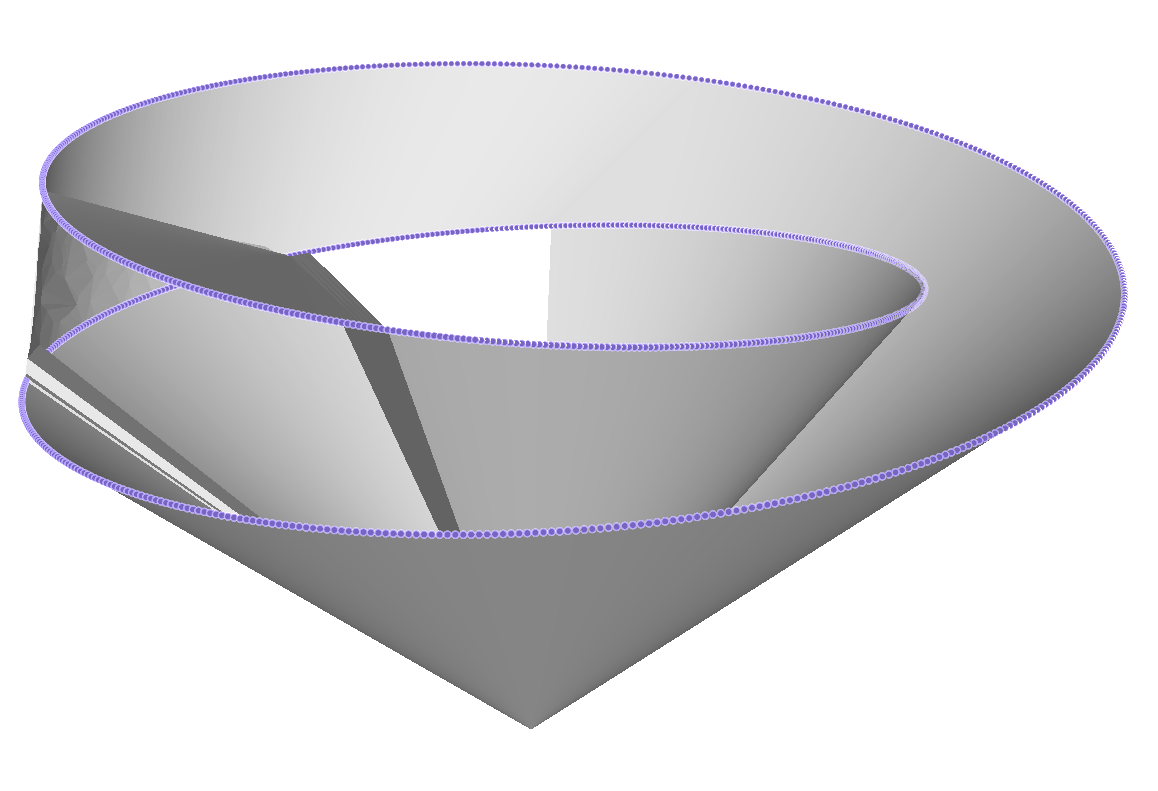
\includegraphics[width=0.32\textwidth]{applications/mobius-representative}};
			\node[below=0cm of rep]{Representative chain};
		\end{tikzpicture}}%
		\visible<3->{%
		\begin{tikzpicture}
			\centering
			\node(result){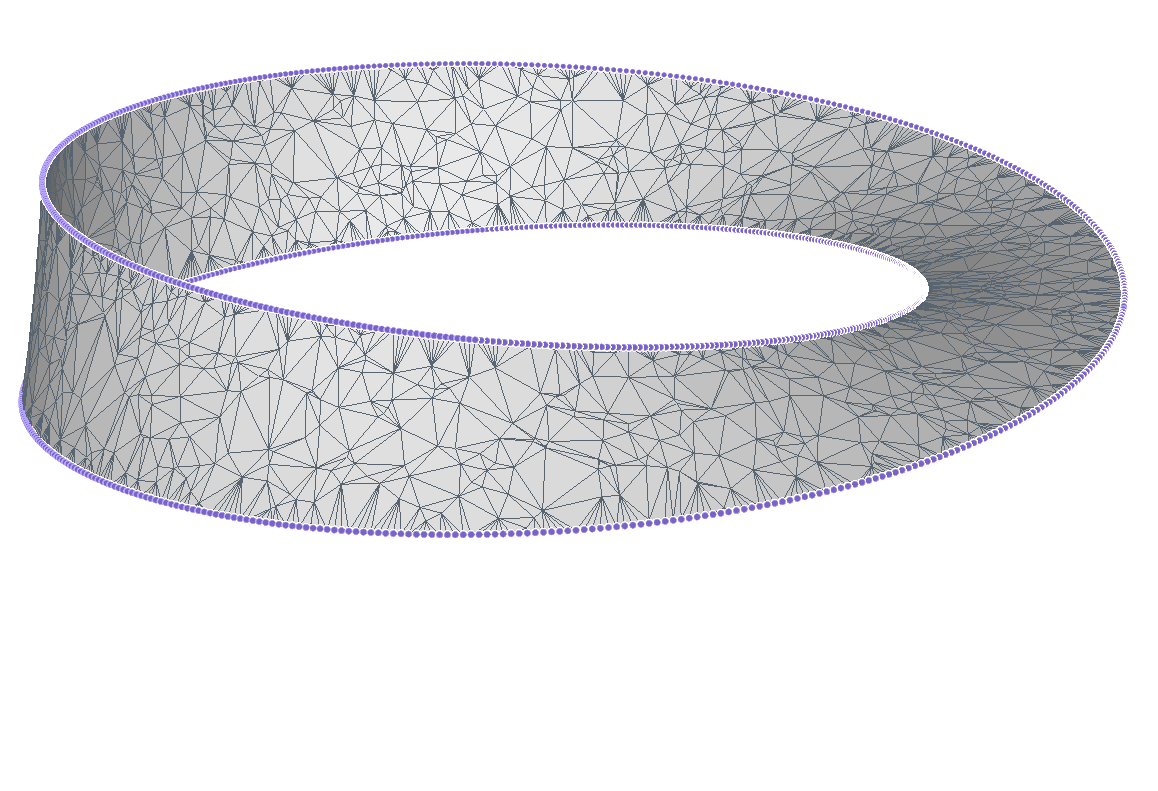
\includegraphics[width=0.32\textwidth]{applications/mobius-optimal}};
			\node[below=0cm of result]{Optimal chain};
		\end{tikzpicture}}
	\end{figure}

	\textbf{Two parts algorithm}
	\begin{itemize}
		\item<2->[1.] Compute a representative chain: any $2$-chain $\Gamma_0$ such that $\partial\Gamma_0$ is the imposed boundary $A$.
		\item<3->[2.] Compute the lexicographic optimal chain homologous to $\Gamma_0$
	\end{itemize}
\end{frame}

\begin{frame}{Part 1: Solution in the Delaunay triangulation}
	\small
	\textbf{Idea:} Recursively replace the highest vertex on the boundary $A$ by edges in its lower link.
	\begin{figure}
		\centering
		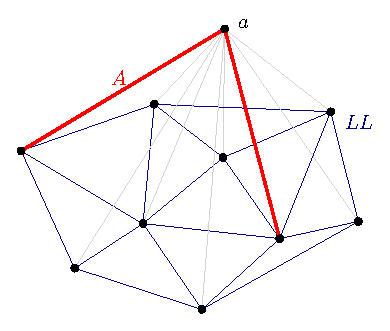
\includegraphics[width=0.32\linewidth]{representative/LowerStar_PathBeforeStep}
		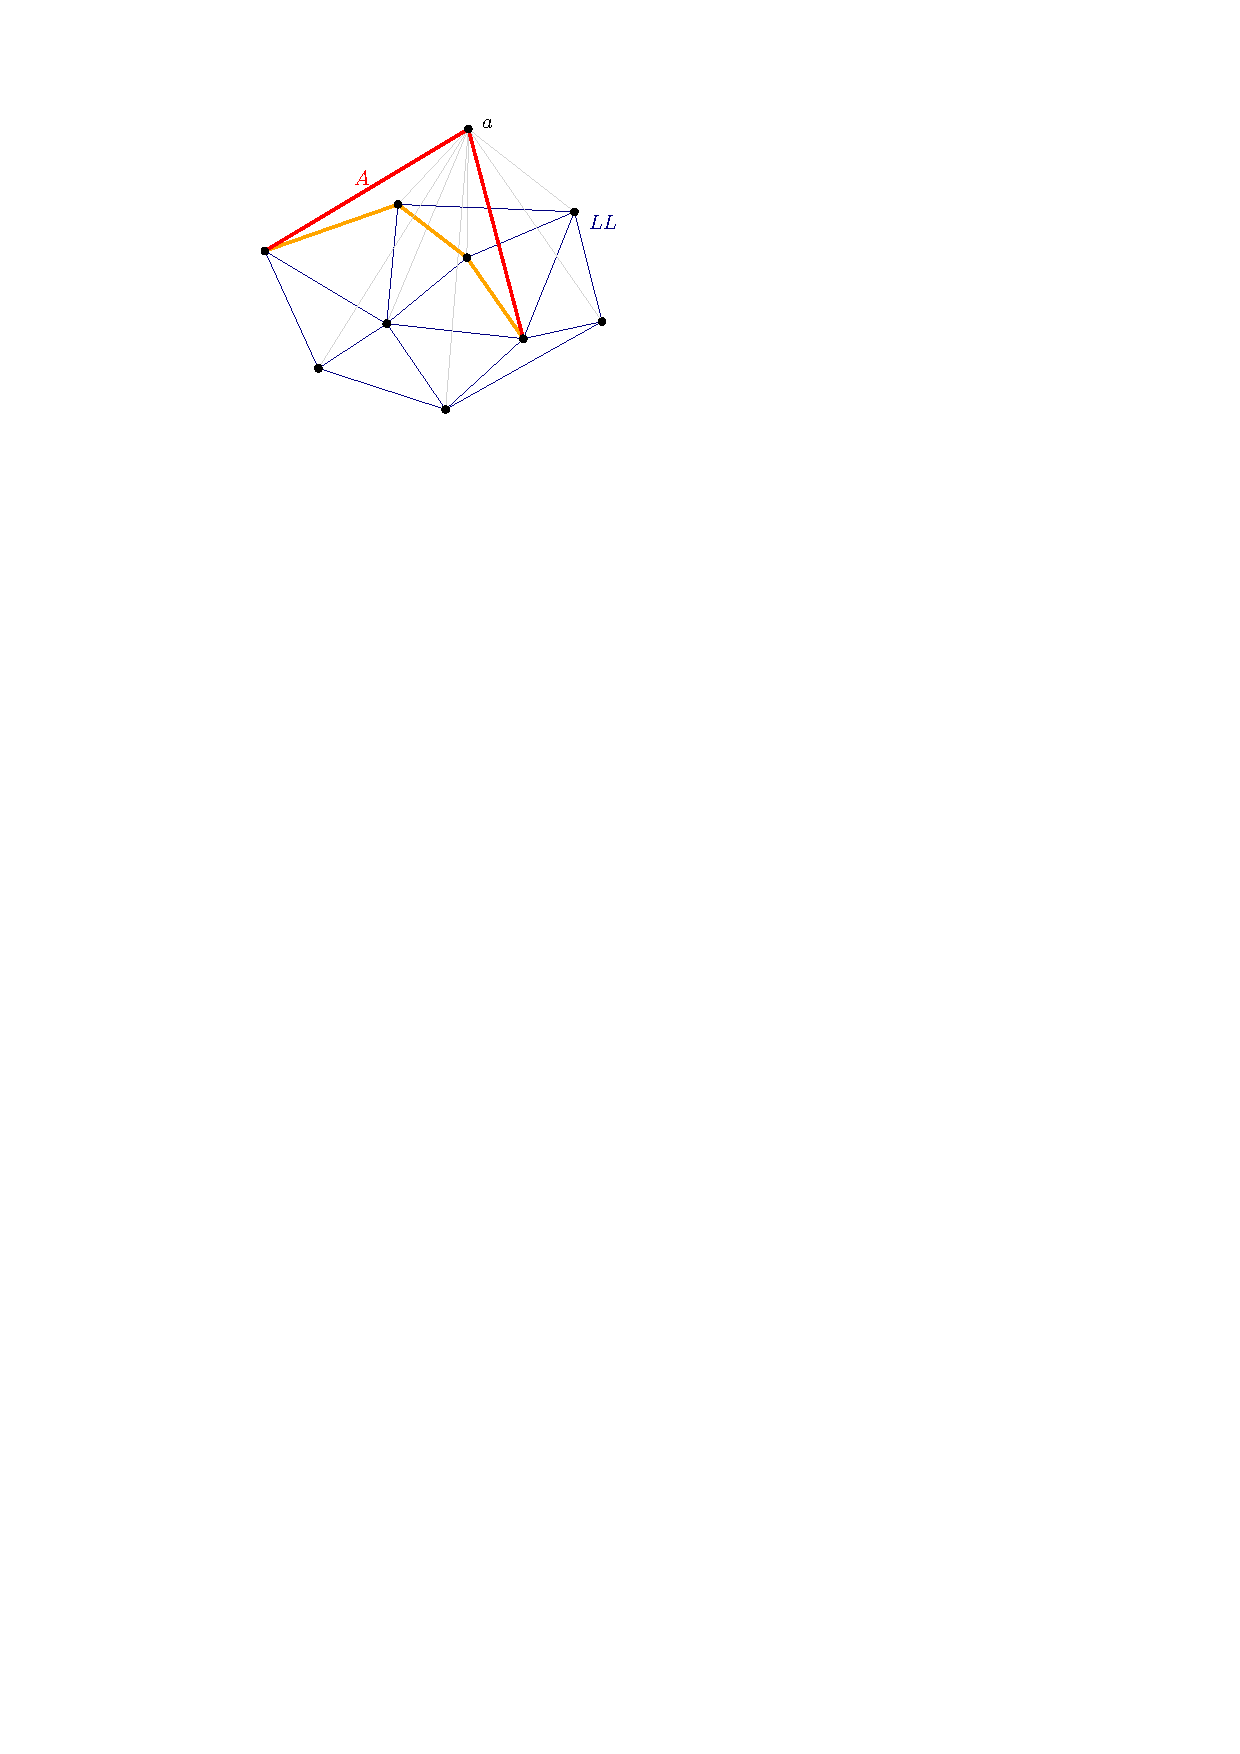
\includegraphics[width=0.32\linewidth]{representative/LowerStar_PathInLink}
		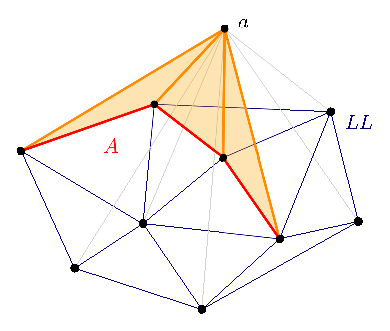
\includegraphics[width=0.32\linewidth]{representative/LowerStar_PathAfterStep}
	\end{figure}

	\textbf{Time complexity: } $\BigO(n \log n)$
\end{frame}


%\begin{frame}{Duality and intersection product}
%
%	
%	\textbf{Orthogonal complement}	
%	\begin{equation}
%		V^{\perp} \defunder{=} \Big\{ \Gamma \in\Cchains_{d-1}(K, B) \mid \forall \gamma \in V, \: \Gamma \otimes \gamma = 0 \Big\}
%	\end{equation}
%\end{frame}

\begin{frame}{Part 2: Optimal homologous chain to $\Gamma_0$}
	\scriptsize
	
	\textbf{Intersection product}
	\begin{align*}
		\begin{split}
			\otimes : \Cchains_2(K) \times  \Cchains_1(\widetilde{K}) &\to \F\\
			(\Gamma, \gamma) &\mapsto \Gamma \otimes \gamma \defunder{=} \sum_{\sigma \in K^{(k)}} \Gamma(\sigma) \: \gamma (\widetilde{\sigma})
		\end{split}
	\end{align*}
	
	\pause
	\textbf{Lefschetz duality}		
	\begin{center}
		\scalebox{0.7}{
			\begin{tikzpicture}
				\small
				\node (duality){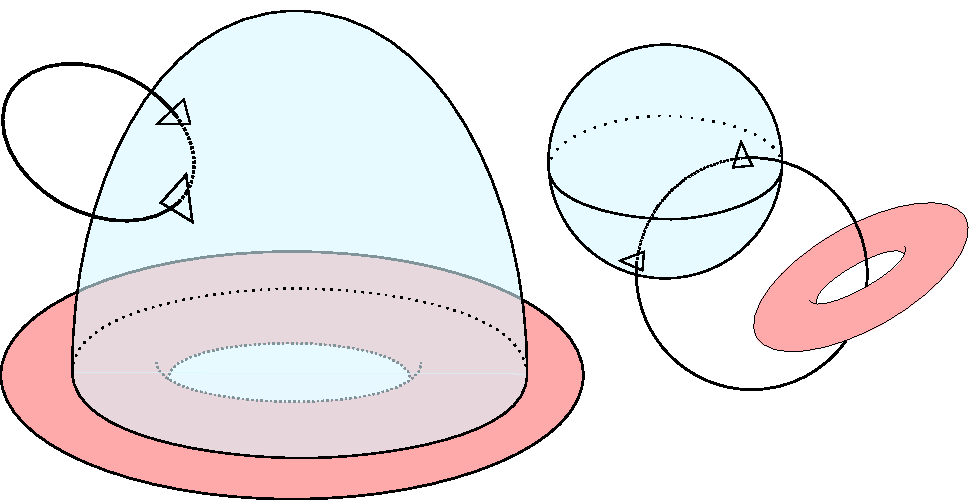
\includegraphics[width=0.7\linewidth]{dual/intersection_product}};
				\node[above left=-0.5cm and -1cm of duality]{$\beta \in \Bchains_1(\widetilde{K \setminus B})$};
				\node[above=-0.3cm of duality]{$\Gamma \in \Zchains_2(K, B)$};
				\node[below right=-1cm and -1.5cm of duality]{$\alpha \in \Zchains_1(\widetilde{K \setminus B})$};
				\node[above right=-1cm and -1.5cm of duality]{$\Delta \in \Bchains_2(K, B)$};
			\end{tikzpicture}
		}
	\end{center}

	\begin{eqnarray*}
		\Gamma \textrm{ homologous to } \Gamma_0 &\iff& \Gamma - \Gamma_0 \in \Bchains_2(K, B) \\
		&\iff& \forall \alpha \in \Zchains_1(\widetilde{K \setminus B}), \; (\Gamma - \Gamma_0) \otimes \alpha = 0
	\end{eqnarray*}
\end{frame}


\begin{frame}{Augmented disjoint-sets structure (A.D.S.)}
	Adds a value in $\F$ to each parent pointer.
	\begin{figure}
		\centering
		\begin{subfigure}{0.45\textwidth}
			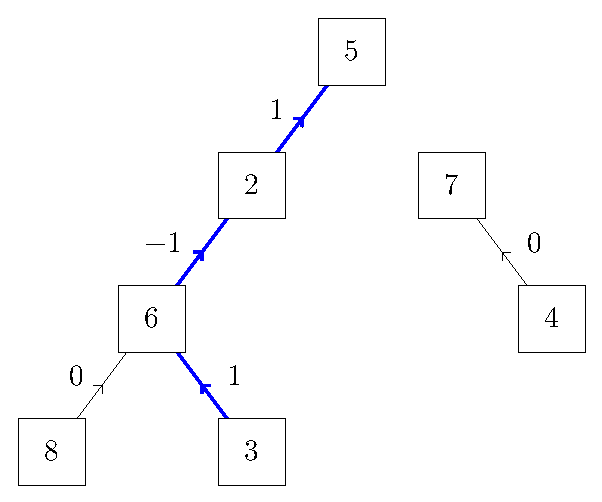
\includegraphics[width=\linewidth]{ds/augmented_disjoint_find}
			\subcaption*{\MFindSet{$3$} $\rightarrow (5, 1)$}
		\end{subfigure}%
		\hspace{0.045\textwidth}%
		\vline%
		\hspace{0.045\textwidth}%
		\begin{subfigure}{0.45\textwidth}
			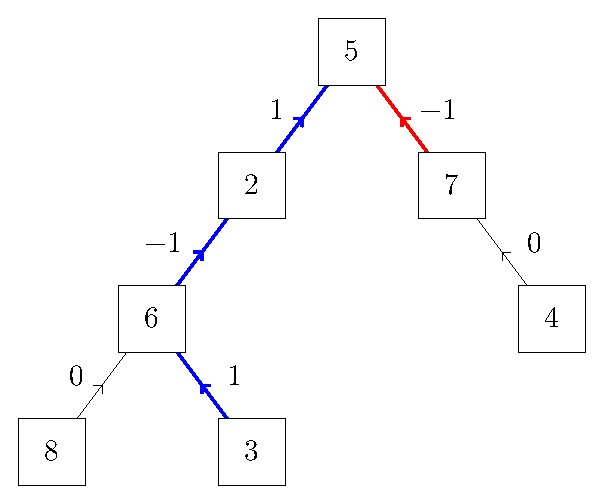
\includegraphics[width=\linewidth]{ds/augmented_disjoint_link}
			\subcaption*{\MLinkSet{$5, 7, -1$}}
		\end{subfigure}%
	\end{figure}
\end{frame}

\begin{frame}{Efficient intersection product computation}
	\small
	\[
		\forall \alpha \in \Zchains_1(\widetilde{K \setminus B}), \; (\Gamma_{\min} - \Gamma_0) \otimes \alpha = 0
	\]
	
	\pause
	\textbf{Algorithm invariants}
	\begin{itemize}
		\item[$\bullet$] For any edge $e$ in the A.D.S., $\Gamma_{\min}(e) = 0$
		\item[$\bullet$] Each edge $e$ in the A.D.S. stores $\Gamma_0 \otimes e$.
	\end{itemize}
		
	\pause
	\begin{minipage}{0.45\linewidth}
		\centering
		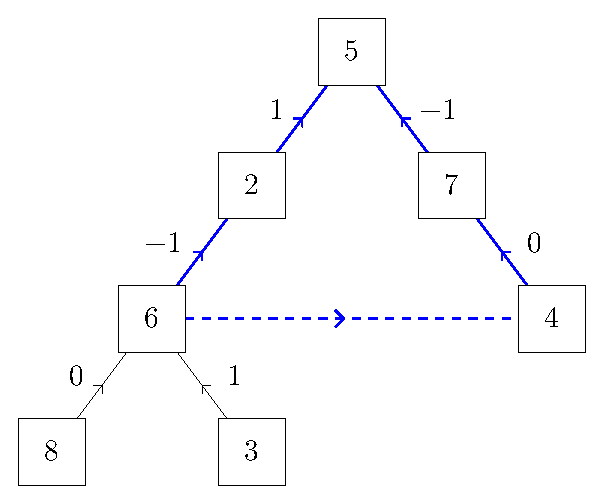
\includegraphics[width=\linewidth]{ds/augmented_disjoint_cycle}
	\end{minipage}%
	\hfill
	\begin{minipage}{0.45\linewidth}
	\pause $(r_1, g_1) \leftarrow$ \MFindSet{$6$}\\
	\pause $(r_2, g_2) \leftarrow$ \MFindSet{$4$}\\
	\pause \begin{eqnarray*} 
				\Gamma_{\min}(e) &=& \Gamma_0 \otimes {\color{blue}\alpha}  \\
								 &=& \Gamma_0(e) + g_2 - g_1
			\end{eqnarray*}
	\end{minipage}
\end{frame}
%
%\begin{frame}{Optimal homologous relative chain}
%	\begin{minipage}{0.7\linewidth}
%		\begin{algorithm}[H]
%			\scriptsize
%			\SetKwInOut{Input}{Inputs}
%			\SetKwInOut{Output}{Output}
%			\SetKw{Continue}{continue}
%				
%			\Input{$\Gamma_0 \in\Cchains_{d-1}(K, B)$.}
%			\Output{$\Gamma_{\min} \in\Cchains_{d-1}(K, B)$, lexicographic optimal relative chain homologous to $\Gamma_0$.}
%			$\Gamma_{\min} \leftarrow 0$ \\
%			\For{$v \in \GraphV_{K \setminus B}$} {
%				\MMakeSet{$v$}
%			}
%			\For{$e \in \GraphE_{K \setminus B}$ in decreasing order}{
%				$e = (v_1, v_2) \in \GraphV_{K \setminus B} \times \GraphV_{K \setminus B}$ \\
%				$(r_1,  g_1) \leftarrow $ \MFindSet{$v_1$}\\
%				$(r_2,  g_2) \leftarrow $ \MFindSet{$v_2$}\\
%				$\alpha = {\Gamma_0}(\widetilde{e}) + g_2 - g_1$\\
%				\uIf{$r_1=r_2$}
%				{$\Gamma_{\min} \leftarrow \Gamma_{\min} + \alpha \cdot \widetilde{e}$}
%				\uElse
%				{\MLinkSet{$r_1$, $r_2$, $\alpha$}}
%			}
%		\end{algorithm}
%	\end{minipage}
%\end{frame}

\begin{frame}{Applications}
	\tiny
	
	\begin{center}
		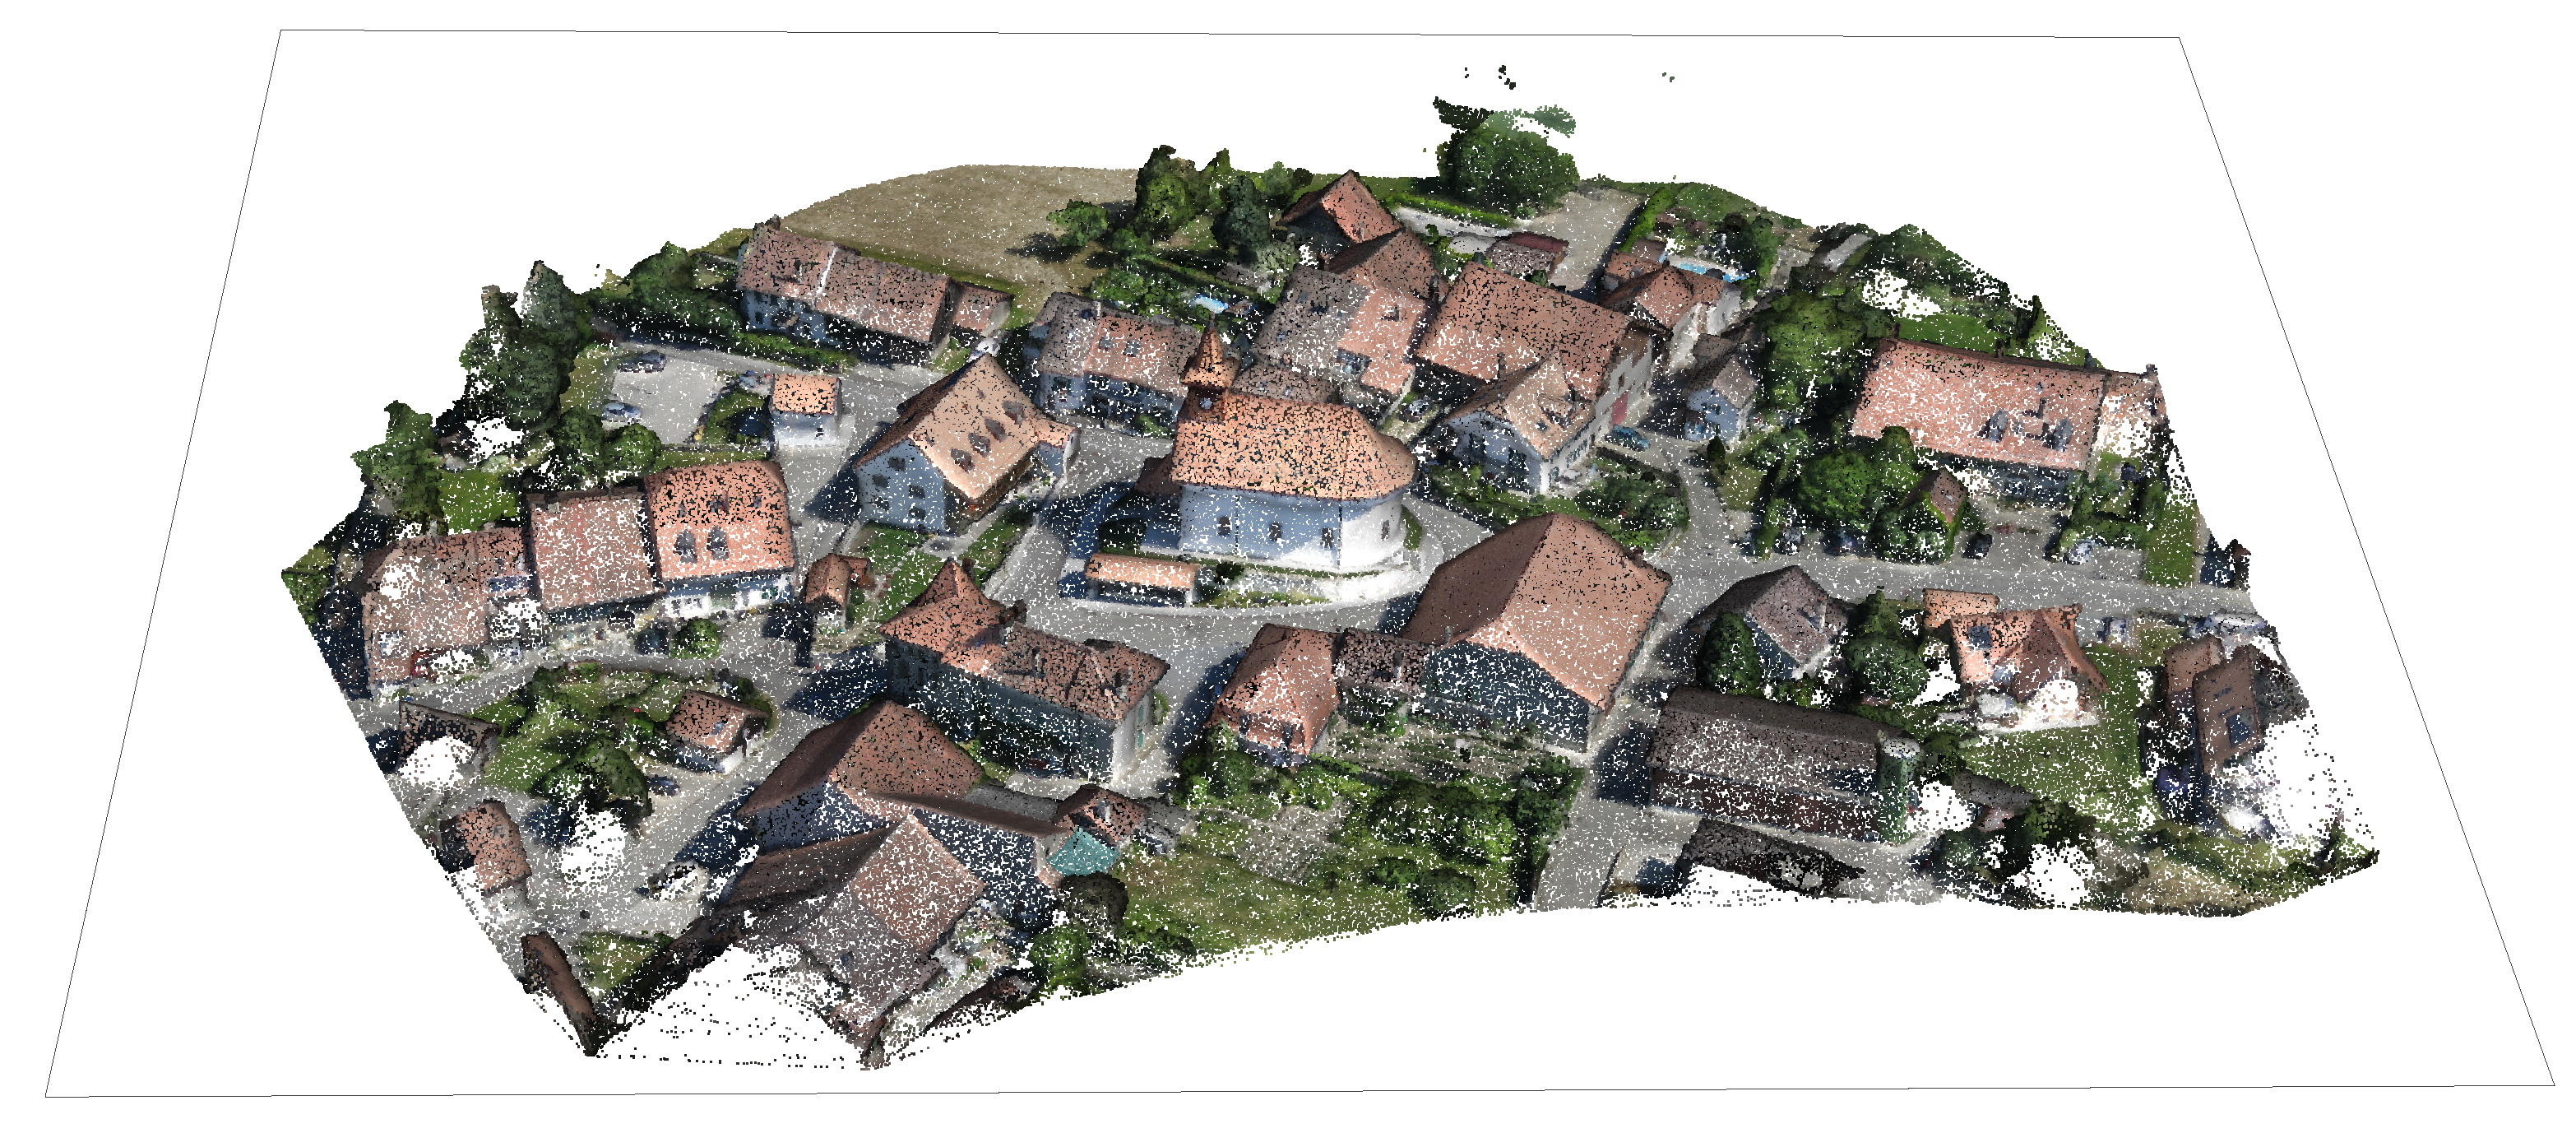
\includegraphics[width=0.49\linewidth]{applications/sullens_points}%
		\includegraphics[width=0.49\linewidth]{applications/sullens_mesh}
		
		\includegraphics[width=0.49\linewidth]{applications/thammasat_points}%
		\includegraphics[width=0.49\linewidth]{applications/thammasat_mesh}
	\end{center}

	\begin{table}
		\centering
		\begin{tabular}{|l|l|l|}  \hline
			\multicolumn{3}{ |c| }{Input} \\ \hline
			Number of points & 1 056 038 & 5 225 819 \\ \hline
			\multicolumn{3}{ |c| }{Performance} \\ \hline
			Delaunay triangulation & 2 633 ms & 14 416 ms \\
			Representative chain & 27 ms & 5 ms \\
			Optimal chain & 1 548 ms & 8 040 ms \\ \hline
		\end{tabular}
	\end{table}
\end{frame}

\begin{frame}{Critical basis}
	\small
	
	\textbf{Lexicographic minimal representative}
	\[
		\Mlex : \Gamma \in \Cchains_k(K, B) \mapsto \min_{\LexicographicOrderChain} \: \Gamma + \Bchains_{k}(K, B)
	\]
	
	$\Mlex$ is \textbf{linear}.
	
	\textbf{Vector space of lexicographic optimal chains}
	\begin{eqnarray*}
		\ZchainMin_k(K,B) &\defunder{=}& \Mlex(\Zchains_k(K, B)) \\
						  &\simeq& \Homol_k(K, B)
	\end{eqnarray*}
	
	\textbf{Critical basis} of $\ZchainMin_k(K,B)$
	\begin{equation*}
		\CritBasis_{i+1} = \min_{\LexicographicOrderChain} \left\{  \Gamma \in  \ZchainMin_k(K) \: \mid \:   \Gamma \notin \Vspan(  \CritBasis_1, \ldots , \CritBasis_i ) \text{ and } \Gamma\big(\Crit(\Gamma)\big)= 1 \right\}
	\end{equation*}
\end{frame}

%\begin{frame}{Critical basis}
%	\small	
%	For $\Gamma \in \ZchainMin_k(K,B)$,
%	\[
%	\Crit(\Gamma) \defunder{=} \max | \Gamma |
%	\]
%	
%	\pause
%	\textbf{Critical basis}
%	\begin{equation*}
%		\CritBasis_{i+1} = \min_{\LexicographicOrderChain} \left\{  \Gamma \in  \ZchainMin_k(K) \: \mid \:   \Gamma \notin \Vspan(  \CritBasis_1, \ldots , \CritBasis_i ) \text{ and } \Gamma\big(\Crit(\Gamma)\big)= 1 \right\}
%	\end{equation*}
%		
%	\pause
%	\begin{center}
%		$\CritBasis_j ( \Crit( \CritBasis_i ) ) =  \delta_{ij}$ where $\delta_{ij}$ is the Kronecker delta. 
%	\end{center}
%
%\end{frame}

\begin{frame}{Applications}
	\scriptsize

	$K$: Delaunay complex of a set of points\\
	$B$: Sharp edge detection (Voronoi Covariance Measure \cite{merigot_VoronoiBasedCurvatureFeature_2011})\\
	
	\vspace{0.5cm}
	\pause
	\begin{minipage}{0.5\linewidth}
		\centering
		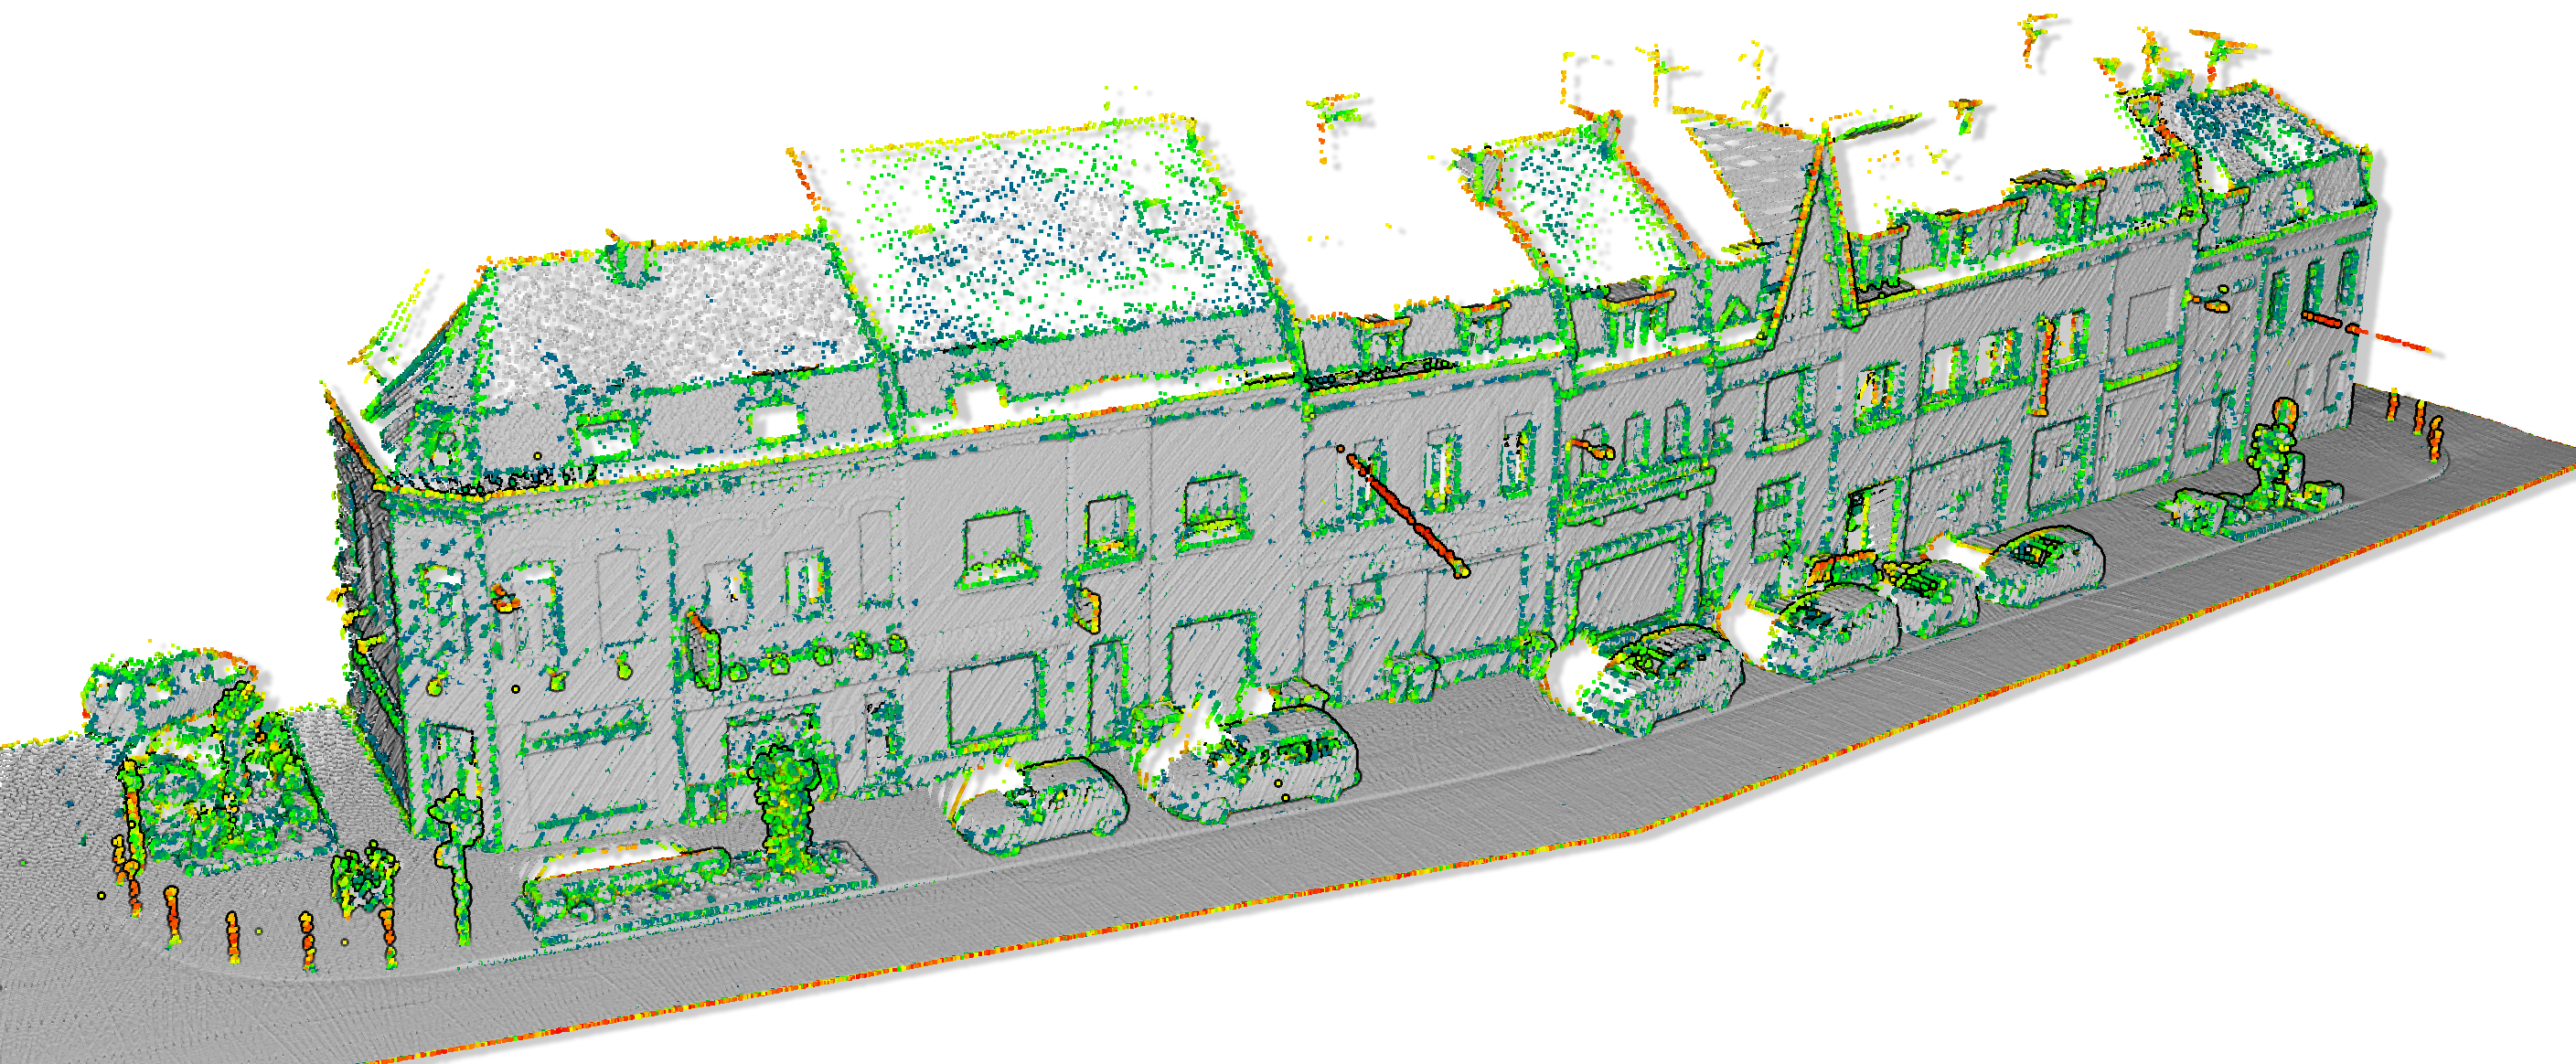
\includegraphics[width=\linewidth]{applications/lille_points}\\
		Sharp feature estimation
	\end{minipage}%
	\hfill%
	\pause%
	\begin{minipage}{0.5\linewidth}
		\centering
		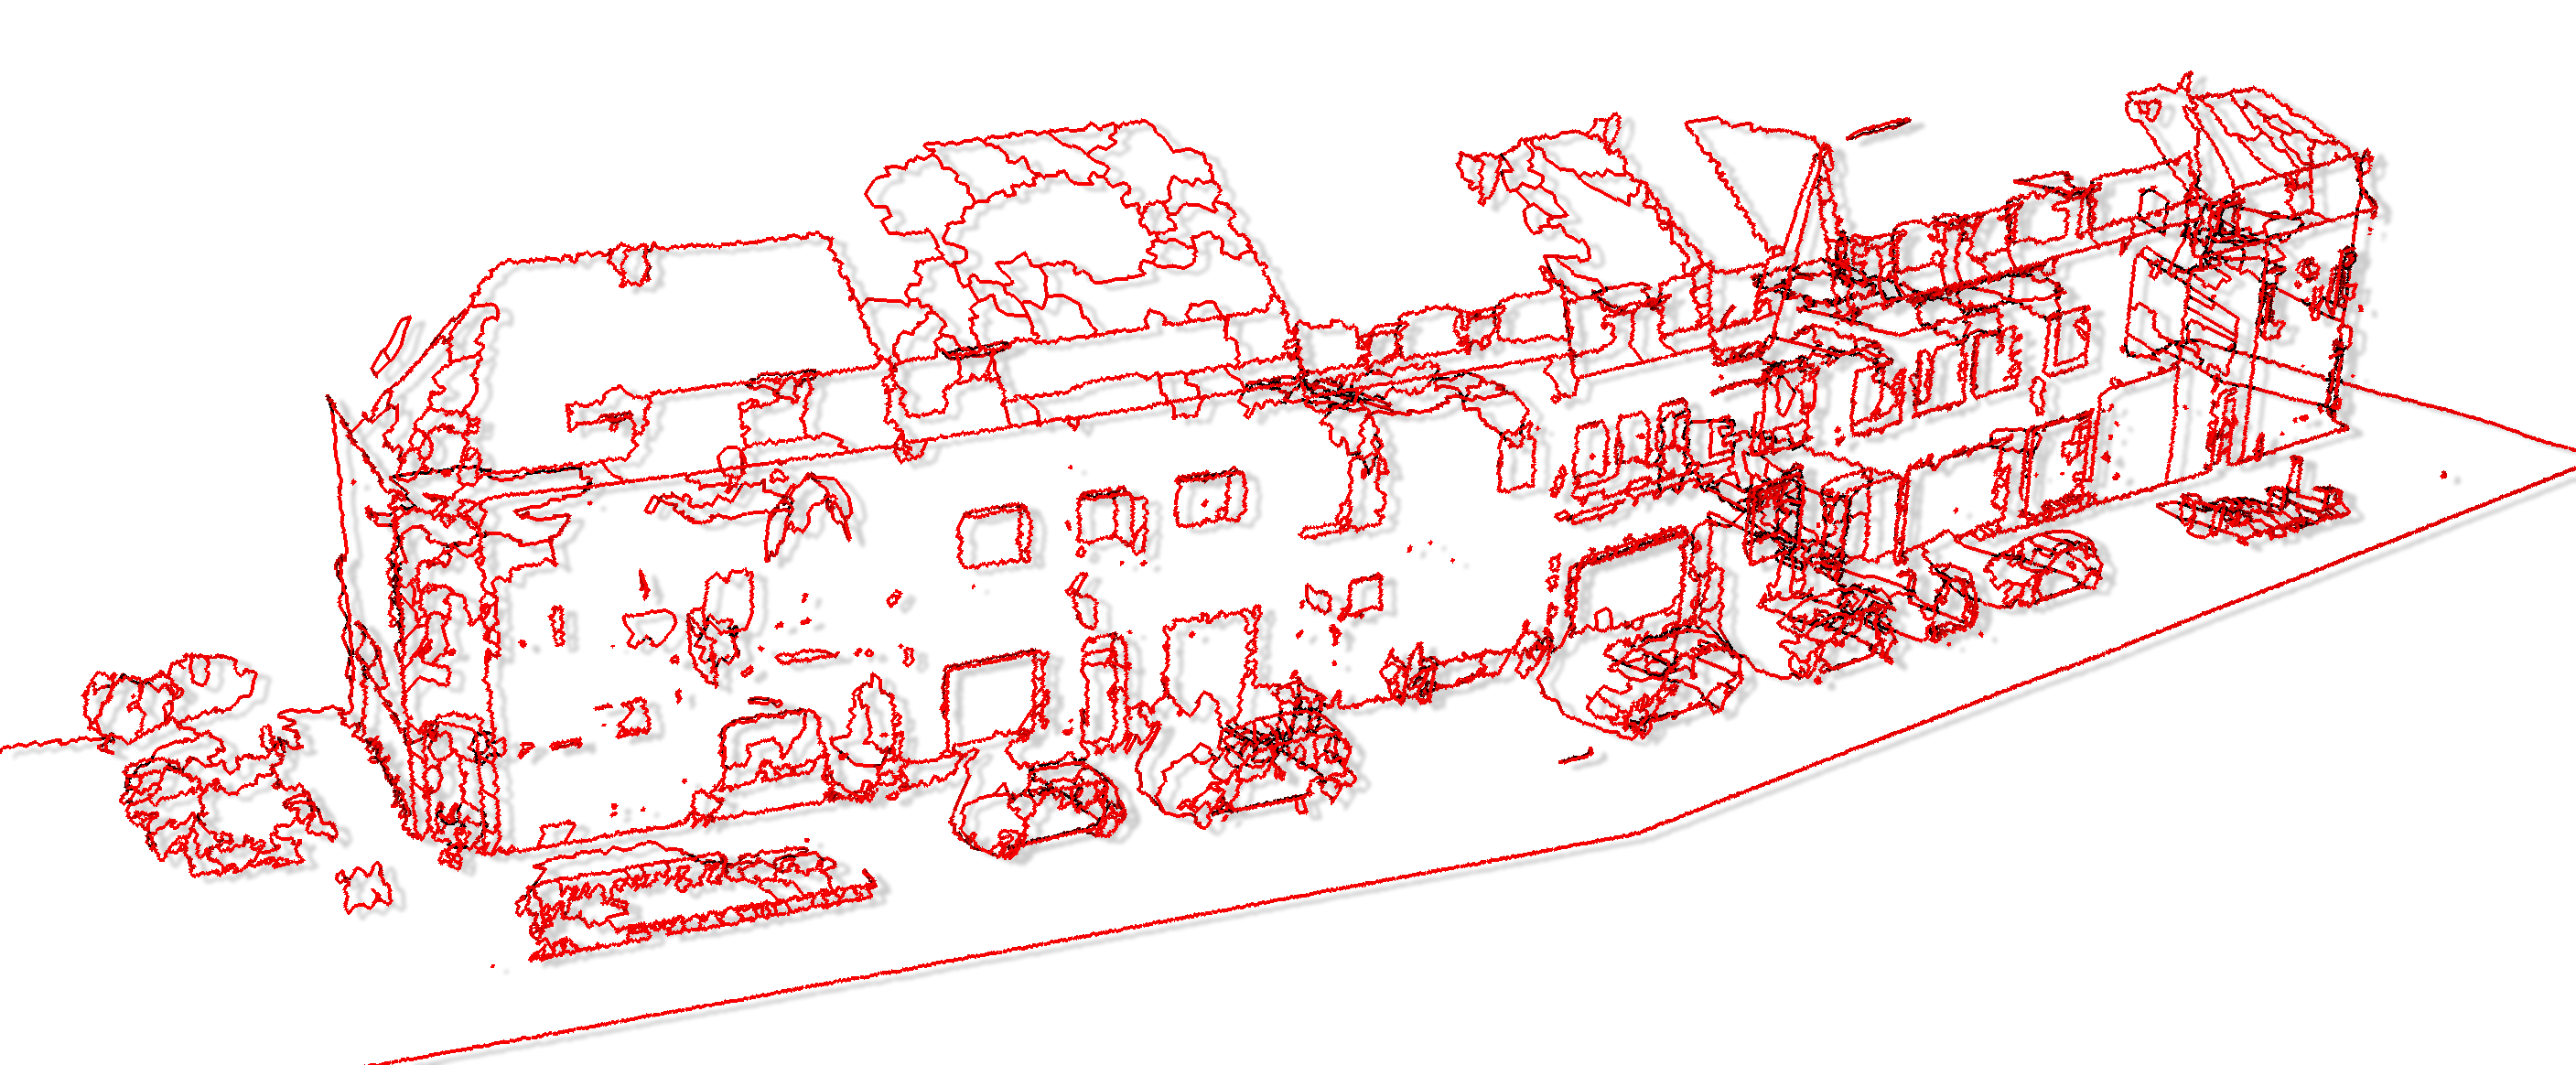
\includegraphics[width=\linewidth]{applications/lille_cycles}\\
		Cycle basis of $\ZchainMin_1(B)$
	\end{minipage}
	
	\pause%
	\begin{minipage}{0.5\linewidth}
		\centering
		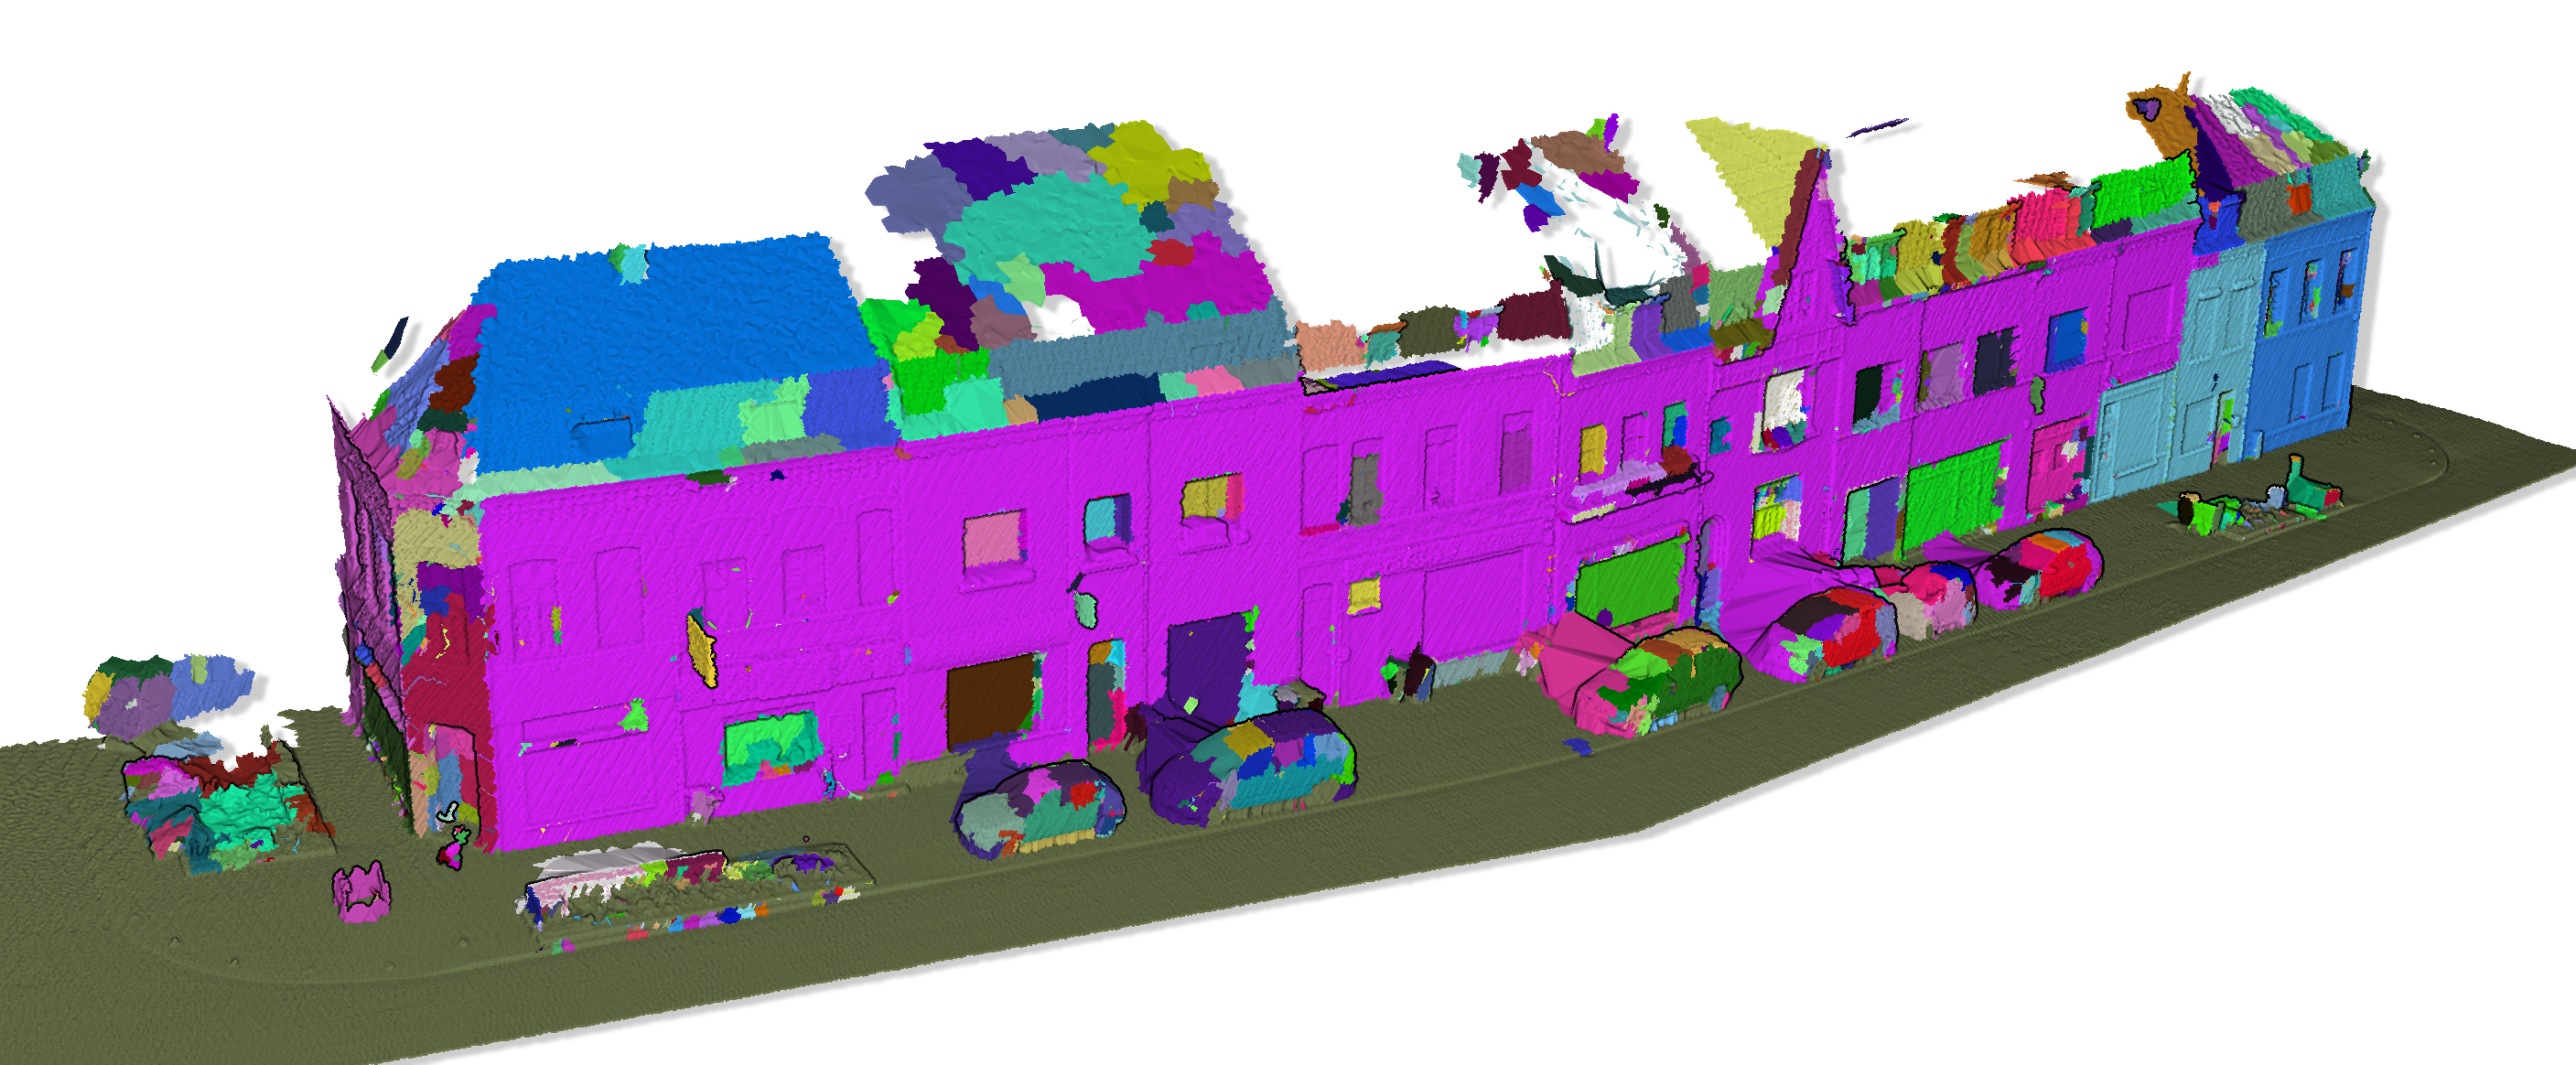
\includegraphics[width=\linewidth]{applications/lille_meshes}\\
		Critical basis of $\ZchainMin_2(K, B)$
	\end{minipage}%
	\hfill%
	\pause%
	\begin{minipage}{0.5\linewidth}
		\centering
		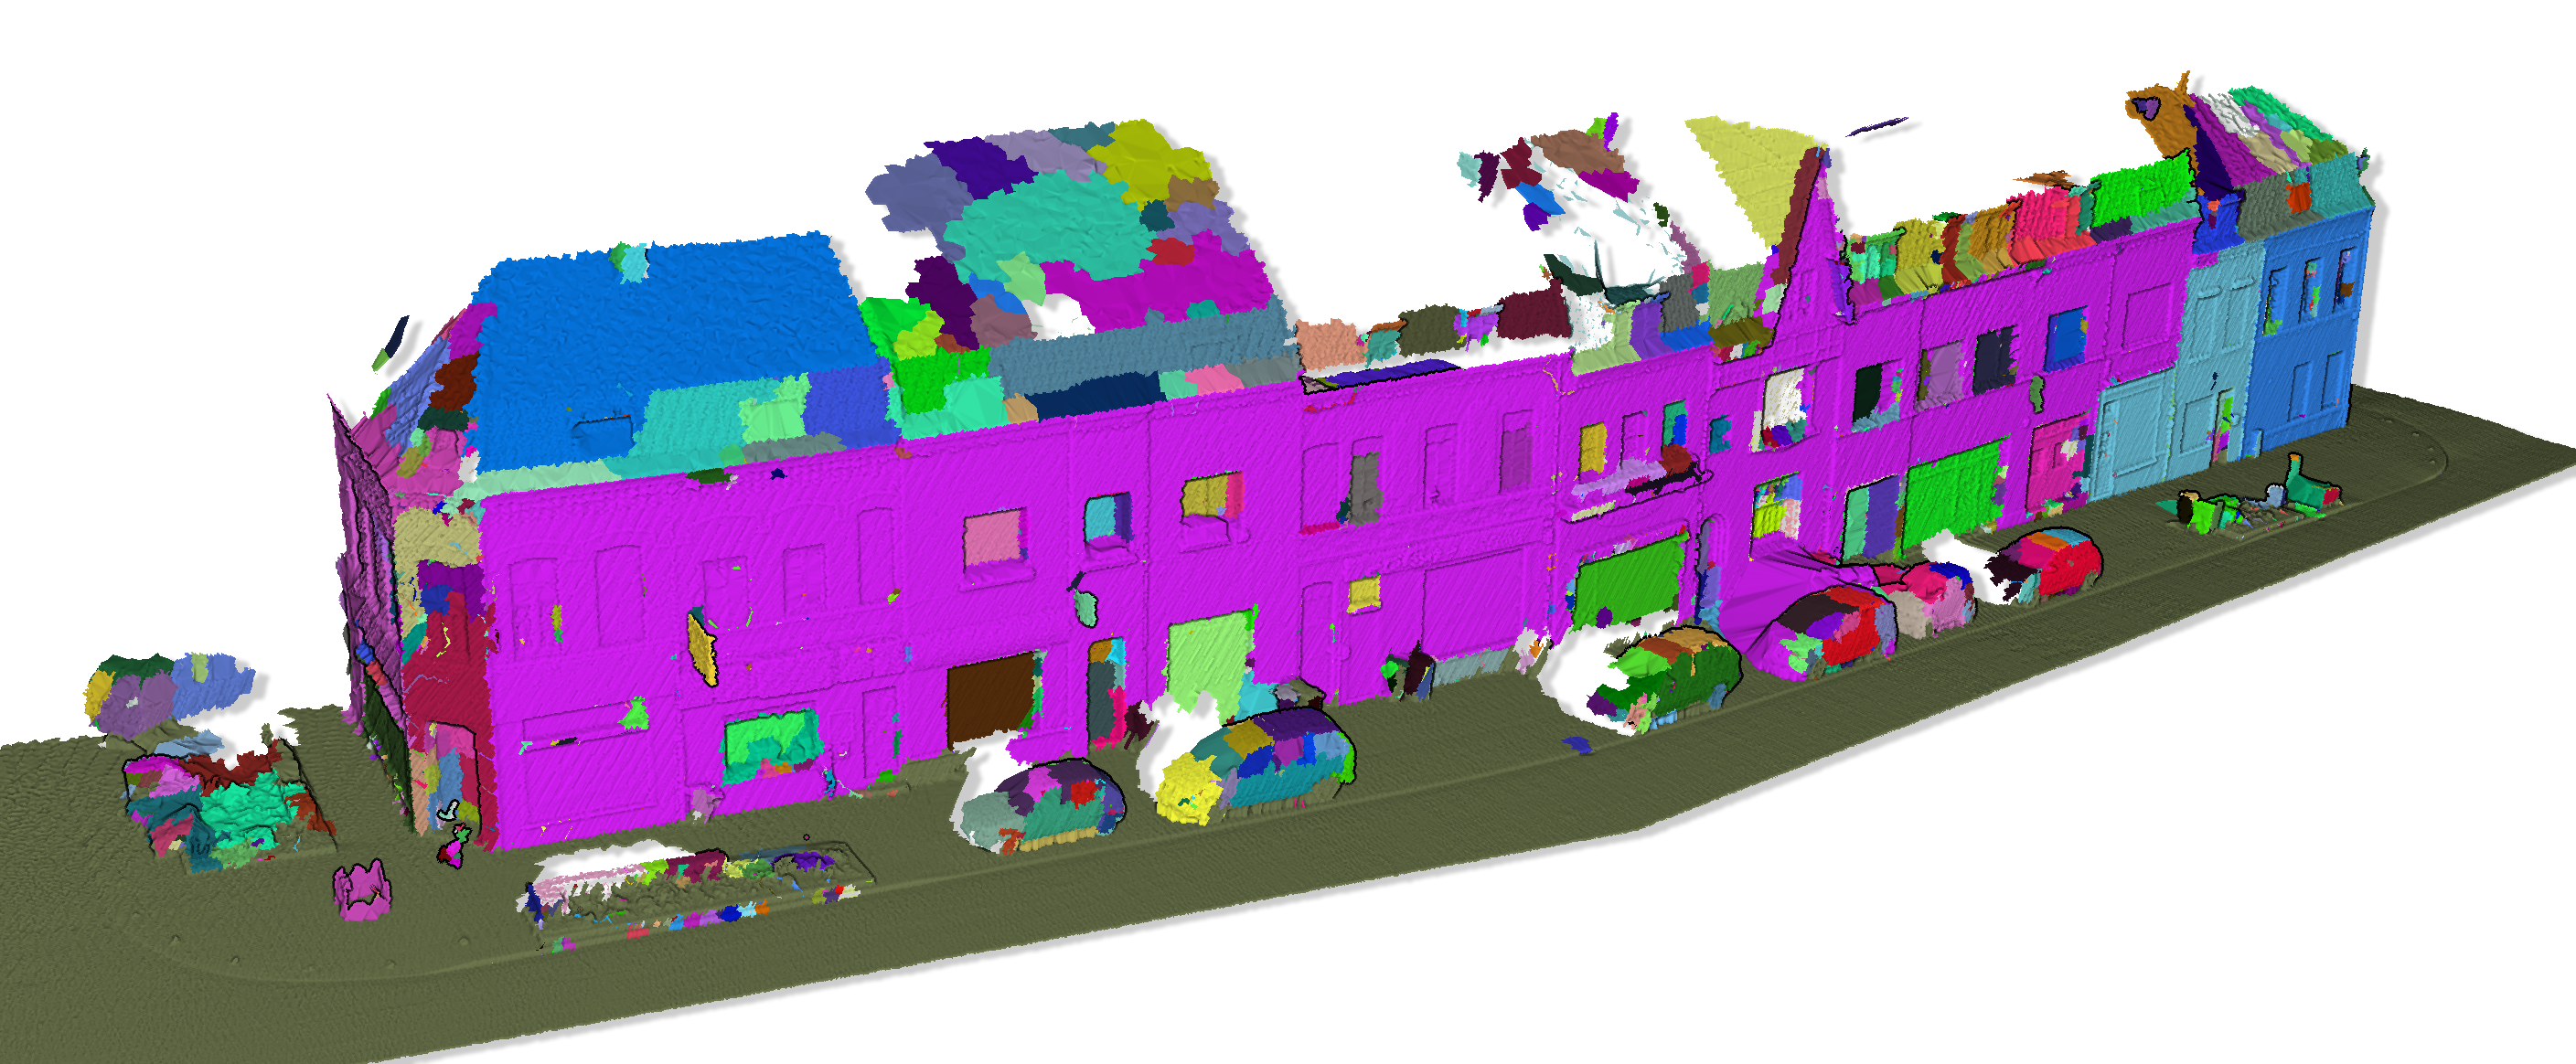
\includegraphics[width=\linewidth]{applications/lille_meshes_2}\\
		Removing the first few chains
	\end{minipage}
\end{frame}